%%
%% Copyright 2007, 2008, 2009 Elsevier Ltd
%%
%% This file is part of the 'Elsarticle Bundle'.
%% ---------------------------------------------
%%
%% It may be distributed under the conditions of the LaTeX Project Public
%% License, either version 1.2 of this license or (at your option) any
%% later version.  The latest version of this license is in
%%    http://www.latex-project.org/lppl.txt
%% and version 1.2 or later is part of all distributions of LaTeX
%% version 1999/12/01 or later.
%%
%% The list of all files belonging to the 'Elsarticle Bundle' is
%% given in the file `manifest.txt'.
%%

%% Template article for Elsevier's document class `elsarticle'
%% with numbered style bibliographic references
%% SP 2008/03/01
%%
%%
%%
%% $Id: elsarticle-template-num.tex 4 2009-10-24 08:22:58Z rishi $
%%
%%
%%%%%\documentclass[preprint,12pt]{elsarticle}

%% Use the option review to obtain double line spacing
%%  \documentclass[preprint,review,12pt]{elsarticle}

%% Use the options 1p,twocolumn; 3p; 3p,twocolumn; 5p; or 5p,twocolumn
%% for a journal layout:
 \documentclass[final,1p,times]{elsarticle}
%% \documentclass[final,1p,times,twocolumn]{elsarticle}
%% \documentclass[final,3p,times]{elsarticle}
%% \documentclass[final,3p,times,twocolumn]{elsarticle}
%% \documentclass[final,5p,times]{elsarticle}
%%\documentclass[final,5p,times,twocolumn]{elsarticle}%%DOS COLUMNAS

%% if you use PostScript figures in your article
%% use the graphics package for simple commands
%% \usepackage{graphics}
%% or use the graphicx package for more complicated commands
%% \usepackage{graphicx}
%% or use the epsfig package if you prefer to use the old commands
%% \usepackage{epsfig}

%% The amssymb package provides various useful mathematical symbols
\usepackage{amssymb}
\usepackage{url}
\usepackage{graphicx}
%% The amsthm package provides extended theorem environments
%% \usepackage{amsthm}

%% The lineno packages adds line numbers. Start line numbering with
%% \begin{linenumbers}, end it with \end{linenumbers}. Or switch it on
%% for the whole article with \linenumbers after \end{frontmatter}.
%% \usepackage{lineno}

%% natbib.sty is loaded by default. However, natbib options can be
%% provided with \biboptions{...} command. Following options are
%% valid:

%%   round  -  round parentheses are used (default)
%%   square -  square brackets are used   [option]
%%   curly  -  curly braces are used      {option}
%%   angle  -  angle brackets are used    <option>
%%   semicolon  -  multiple citations separated by semi-colon
%%   colon  - same as semicolon, an earlier confusion
%%   comma  -  separated by comma
%%   numbers-  selects numerical citations
%%   super  -  numerical citations as superscripts
%%   sort   -  sorts multiple citations according to order in ref. list
%%   sort&compress   -  like sort, but also compresses numerical citations
%%   compress - compresses without sorting
%%
%% \biboptions{comma,round}

% \biboptions{}


\journal{Expert Systems with Applications}

\begin{document}

\begin{frontmatter}

%% Title, authors and addresses

%% use the tnoteref command within \title for footnotes;
%% use the tnotetext command for the associated footnote;
%% use the fnref command within \author or \address for footnotes;
%% use the fntext command for the associated footnote;
%% use the corref command within \author for corresponding author footnotes;
%% use the cortext command for the associated footnote;
%% use the ead command for the email address,
%% and the form \ead[url] for the home page:
%%
%% \title{Title\tnoteref{label1}}
%% \tnotetext[label1]{}
%% \author{Name\corref{cor1}\fnref{label2}}
%% \ead{email address}
%% \ead[url]{home page}
%% \fntext[label2]{}
%% \cortext[cor1]{}
%% \address{Address\fnref{label3}}
%% \fntext[label3]{}

\title{Using SOAP and REST web services as communication protocol for distributed evolutionary computation}
%SOAP and REST Web Services for Distributed Evolutionary Computation Implementation
%\titlerunning{ short title}

\author[ugr]{P.A. Castillo}
  \ead{pacv@ugr.es}
\author[ugr]{P. Garc\'{\i}a-S\'{a}nchez}
  \ead{pgarcia@atc.ugr.es}
\author[ugr]{M.G. Arenas}
  \ead{mgarenas@ugr.es}
\author[ugr]{G. Romero}
  \ead{gustavo@ugr.es}
\author[ugr]{A.M. Mora}
  \ead{amorag@geneura.ugr.es}
\author[ugr]{J.J. Merelo}
  \ead{jmerelo@geneura.ugr.es}

\address[ugr]{Department of Computer Architecture and Computer Technology and CITIC-UGR, University of Granada, Granada, Spain. Tel: +34958240589. Fax: +34958248993}
%\address[upv]{Institute of Advanced ICT, Polytechnic University of Valencia, Valencia, Spain}
%\address[jam]{Jambit GmbH, Munich, Germany}

%%%%%%%%%%%%%%%%%%%%%%%%%%%%%%%%%%%%%%%%%%%%%%%%%%%%%%%%%%%%%%%%%%%%%%%%%%%%%%%%%%%%%%%%%
%%%%%%%%%%%%%%%%%%%%%%%%%%%%%%%%%%%%%%%%%%%%%%%%%%%%%%%%%%%%%%%%%%%%%%%%%%%%%%%%%%%%%%%%%
%%%%%%%%%%%%%%%%%%%%%%%%%%%%%%%%%%%%%%%%%%%%%%%%%%%%%%%%%%%%%%%%%%%%%%%%%%%%%%%%%%%%%%%%%

\begin{abstract}
In this paper we propose using Simple Object Access Protocol (SOAP) and {REpresentational State Transfer} (REST), two main approaches for creating applications based on distributed services, for distributed computation.
Our aim is to demonstrate how they could be used to develop evolutionary computation systems on heterogeneous platforms, taking advantage of their ability to deal with heterogeneous infrastructures and environments, and giving support for parallel implementations with a high platform flexibility.  
Both approaches are different and present some advantages and disadvantages for interfacing to web services: SOAP is conceptually more difficult (has a steeper learning curve) and more ''heavy-weight'' than REST, although it lacks of standards support for security.
%Although the adoption of a new paradigm is not easy, the importance of the new emerging engineering problems must be taken into account.
%In order to test their efficiency (in time), three experiments have been performed using both technologies: 
%first a basic client-server model implementation to test communications has been implemented;
%then, a master-slave based genetic algorithm (GA) to solve an optimization problem has been used;
%and finally, as third experiment, an approach to evolutionary distributed optimisation of multilayer perceptrons (MLP) using REST and language Perl has been done. 
%In these experiments, a master-slave based evolutionary algorithm (EA) has been implemented, where slave processes evaluate the costly fitness function (training a MLP to solve a classification problem).
%As expected, the parallel version of the developed programs obtains similar or better results using much less time than the sequential version.
The results obtained on different experiments have shown that both SOAP and REST can be used as communication protocol for distributed evolutionary computation. 
Results obtained are comparable, however for large amounts of data (big messages), REST communications take longer than SOAP communications.

\end{abstract}

\begin{keyword}
Simple Object Access Protocol \sep REpresentational State Transfer \sep distributed evolutionary computation
\end{keyword}

\end{frontmatter}


%%%%%%%%%%%%%%%%%%%%%%%%%%%%%%%%%%%%%%%%%%%%%%%%%%%%%%%%%%%%%%%%%%%%%%%%%%%%%%%%%%%%%%%%%
%%%%%%%%%%%%%%%%%%%%%%%%%%%%%%%%%%%%%%%%%%%%%%%%%%%%%%%%%%%%%%%%%%%%%%%%%%%%%%%%%%%%%%%%%
%%%%%%%%%%%%%%%%%%%%%%%%%%%%%%%%%%%%%%%%%%%%%%%%%%%%%%%%%%%%%%%%%%%%%%%%%%%%%%%%%%%%%%%%%

\section{Introduction}
\label{sec:introduction}

Using web services technologies for distributed computation might provide a common interface that can be called from almost any programming language to develop evolutionary computation systems on heterogeneous platforms. 
Services are computational resources that can be utilized and organized through the Service Oriented Architecture (SOA) \cite{PAPAZOGLOU} paradigm. 
In order to use this paradigm, the service providers publish the descriptions (or interfaces) of the services they offer in a service registry, so the service requesters can discover them and bind to the correspondant service provider.

%añadido en la revisión de diciembre-12
An important SOA capability is that it is not focused on a specific implementation, but offers a set of guidelines to help the developers \cite{SOMA}. 
The order of service execution is not necessarily static, because the services are designed to be used in a non-established and configurable order.
Furthermore, services can be dynamically discovered and used (while in Object Oriented Programming must be previously known and can not change during execution), being also one of the most important capabilities the (optional) distribution in a network.

The web services are the key point of integration for different applications belonging to different platforms/languages/systems since they are based in a set of standards that make them independent of the underlying technologies used for providing them.
Although there are several technologies for developing web services
(SOAP, REST or XMLRPC among others \cite{Daigneau2011}),
nowadays the more popular approaches are SOAP  \cite{SOAP} and REST \cite{Fielding2000,Fielding2002,Vinoski2008}.
%Both implementations are suitable for designing web services, however, it is important to understand the pros and cons of each one.

%
%  MIRAR EN:   http://www.infoq.com/news/2011/06/Is-REST-Successful
% si fuese necesario dar estadísticas de uso actualizadas:
%
SOAP is the traditional, standards-based approach, but the majority of the web services with public API offer REST interfaces, while some of them offer both REST and SOAP and very few offer just SOAP.
All of the major web services providers use REST: Twitter, Yahoo's, Flickr, del.icio.us, pubsub, bloglines, technorati, and several others. Both eBay and Amazon have web services for both REST and SOAP.


On the other hand, SOAP web services are used in lots of enterprise software as well; for example, Google implements their web services using SOAP, with the exception of Blogger, which uses XML-RPC, an early and simpler pre-standard of SOAP. 

The philosophies of SOAP and RESTful web services are very different. Strictly, SOAP is a protocol for distributed computing, whereas REST adheres much more closely to a web-based design. 
SOAP requires a greater implementation and understanding effort of the client side, while REST based APIs focus these efforts on the server side. 
%Table \ref{tabla:pro_cons} shows the main strengths and weaknesses for both SOAP and REST.


It is important to note that one of the advantages of SOAP is the use of the ''generic'' transport. While REST today uses HTTP/HTTPS, SOAP can use almost any transport to send the request. 
However, one perceived disadvantage is the use of XML \cite{LearningXML} because of its verbosity, and the time necessary to parse it.

Whatever the technology used to deploy web services, they provide several advantages \cite{GENERICITY05}, like language independence and distribution mechanisms; 
it also increases the interoperability between different software elements (for example, it is possible to add communication libraries without modifying existing code), and facilitates code distribution (it is not required the use of a concrete implementation or library) among geographically distributed work teams.

%añadido en la revisión de diciembre-12
%In scenarios such as GRIDs, several big and expensive processes are being executed, so web services extensions must be applied: contract, security or state management, for example.  Web services are used in the GRID area for optimization problems \cite{GRID1,GRID2,GRID3}, where services are defined using WSDL interfaces and other transmission mechanisms (such as Remote Procedure Call \cite{GRID6}). Although there also exist EAs to be executed in GRIDs (\cite{GRID8,GRID10}) no information about how to design these services for EAs is provided. Implementation technologies, such as Web Services are the gap between SOA (abstract) and GRID (infrastructure) where interfaces are designed using SOA principles (dynamism, visibility, loose-coupling and heterogeneity). Finally, Cloud Computing can be seen as a combination that extends SOA adding the scalability of GRID \cite{SOALIB}. 


%In this paper we propose using SOAP and REST approaches for distributed computation, demonstrating how they could be used to develop evolutionary computation systems on heterogeneous platforms, taking advantage of flexibility, fault tolerance and resilience to infrastructure breakdowns. 
In this paper, a high-level comparison of the SOAP and REST approaches is made. We propose using them for distributed evolutionary computation, taking advantage of their ability to deal with heterogeneous infrastructures and environments.
We intend to innovate in terms of the implementation, because implementation matters \cite{jjiwann2011}, as new technologies lead to new ways of implementing the algorithms, they allow new developers to work on new methods and using many computers on distributed experiments.

In order to determine the efficiency of these two interfacing approaches, we have performed four experiments in which both a SOAP and REST implementations are evaluated, taking a ''toy problem'' as proof of concept, a function optimization problem, and a complex artificial neural network design and optimization problem. 
As first experiment a client-server model is implemented, in which the server process runs on a machine and the client processes send and receive text strings.
Next, a master-slave based genetic algorithm (GA) is implemented, running on the master process the GA and the fitness evaluation on the slave processes.
Then, based on the previous one, a real-coded EA to solve function optimization problems has been tested on three well known functions taken from the CEC2005 benchmark.
Finally, as fourth experiment, we implement a distributed evolutionary algorithm (EA) to solve a costly problem: tuning learning parameters and to set the initial weights and hidden layer size of a multilayer perceptron (MLP), based on an EA and Quick Propagation \cite{FahlmanQP} (QP) to solve classification problems.

This work continues with our previous research in service oriented algorithms, as previously stated in \cite{OSGILIATH}, where a service-oriented platform was presented, or evolutionary optimisation of MLP (G-Prop method) presented in \cite{CastilloNPL},\cite{castilloNC}. 
%\emph{G-Prop} leverages the capabilities of two classes of algorithms: the ability of EA to find a solution close to the global optimum, and the ability of the back-propagation algorithm (BP) to tune a solution and reach the nearest local minimum by means of local search from the solution found by the EA. Instead of using a pre-established topology, the population is initialised with different hidden layer sizes, with some specific operators designed to change them (mutation, multi-point crossover, addition and elimination of hidden units, and QP training applied as operator). The EA searches and optimises the architecture (number of hidden units), the initial weight setting for that architecture and the learning rate for that net.

The main idea of this paper %, which is basically a proof of concept, 
is to study what are the possibilities of this setup as a flexible meta-computer by implementing an EA using web services, and then measuring the speedup when several computers are used to solve a costly classification problem, so that it takes time enough to get some improvement from parallelization. 
We will only measure how running time scales when new (heterogeneous) nodes are added to the system, being the main objective to test if this kind of system is suitable for scientific computation.

\medskip

This paper is structured as follows:
In section \ref{sec:SOAPvsREST} a comprehensive description of SOAP and REST technologies are provided.
Section \ref{sec:soa} presents a review of the approaches found in the bibliography to describe and implement parallel and distributed EA.
Section \ref{sec:experimento} describes the experiments in detail. In concrete, the client-server and master-slave models implemented for testing are described,
as well as the experimental configuration, and the methodology considered in the study; finally, the results obtained are shown.
Last section (Section \ref{sec:conclusionsAndFutureWork}), throws some conclusions and presents the proposed future work.


%%%%%%%%%%%%%%%%%%%%%%%%%%%%%%%%%%%%%%%%%%%%%%%%%%%%%%%%%%%%%%%%%%%%%%%%%%%%%%%%
\section{Comparing SOAP and REST services}
\label{sec:SOAPvsREST}

This section presents a comprehensive description of SOAP (Section \ref{sec:SOAP}) and REST (Section \ref{sec:REST}) technologies, followed by a comparison of SOAP and REST programming models (Section \ref{sec:progmodels}).


%%%%%%%%%%%%%%%%%%%%%%%%%%%%%%%
\subsection{SOAP: Simple Object Access Protocol}
\label{sec:SOAP}

SOAP is a standard protocol proposed by the W3C \cite{SOAP} to interface web  which  extends the XML remote procedure call (XML-RPC) standard. 
SOAP is a complete and mature protocol that allows to perform remote method calls to distributed routines (services) based on an XML interface.

SOAP clients can access to objects and methods that are residing in remote servers, using a standard mechanism that makes transparent the details of implementation, such us the programming language of the
routines, the operating system or the platform used by the provider of the service. 
At the moment, there exist complete implementations of SOAP for Perl, Java, Python, C++ and most modern languages \cite{SOAP:soft}.
In opposite to other remote procedure call methods, such as RMI (\emph{remote method invocation}, used by the Java language) or XML-RPC, SOAP has two main advantages: it can be used with any programming language, and it can use any type of transport (HTTP, SHTTP, TCP, SMTP, POP and other protocols).

SOAP messages are sent using XML. % \cite{LearningXML},\cite{xml:bible}
The interfaces of the methods that can be accessed are specified by a Web Services Description Language (WSDL) \cite{Alonso2010}. %\cite{SOAP:WSDL,SOAP:WSDL2}. 
The WSDL of a web service consists in an XML description of its interface, i.e., it is a file that describes the name of the methods, the parameters (number and type) and the type of response.
%Using an WSDL file, that it is based on a neutral language such as XML, the service can be specified for different languages, so that a Java client can access a Perl server.

In this way, SOAP constitutes a high level protocol, making easy the task of distributing objects among different servers, and avoiding the difficulties derived of defining the message formats, nor the explicit call to remote servers.


One of the advantages of using web services, is that the aplication stack is growing with the WS-Extensions. That is, the basic specifications of Web Services (such as SOAP) can be extended with transactions, security or messaging, for example. The most used are:
\begin{itemize}
  \item WS-Adressing \cite{WSA} (authentication)
  \item WS-Security \cite{WSS}, WS-SecureConversation \cite{WSSC} and WS-Trust \cite{WSTrust} (authorization and secure messaging)
  \item WS-Policy and WS-Metadata Exchange \cite{WSP} (policy mechanisms for interactions)
  \item WS-Reliable Messaging \cite{WSR} and WS-Transaction \cite{WST} (add-on mechanisms for the communication channel)
\end{itemize}

Also, functional extensions, such as WSRF \cite{WSRF}, allows the discovery, inspection and interaction with stateful resources in standard and interoperable ways.

Several studies about e-science taking advantage of web services can be found in bibliography \cite{Taverna,davidson,Kepler,Perera}.
%In \cite{Perera} all these extensions are explained and applied to a large scientific project as example. The authors concluded that extensions can be added even if they were not taking into account when the existent project was designed.


%%%%%%%%%%%%%%%%%%%%%%%%%%%%%%%
\subsection{REST: Representational State Transfer}
\label{sec:REST}

Representational State Transfer (REST)\footnote{\url{http://en.wikipedia.org/wiki/Representational_state_transfer}} is an alternative method for building web services.
This technology was proposed and defined by Roy Fielding \cite{Fielding2000},\cite{Fielding2002}.

%REST is a style of software architecture for distributed hypermedia systems such as the World Wide Web. The term Representational State Transfer was introduced and defined in 2000 by Roy Fielding in his doctoral dissertation \cite{Fielding2000},\cite{Fielding2002}. Fielding is one of the principal authors of the Hypertext Transfer Protocol (HTTP) specification versions 1.0 and 1.1 \cite{wikiREST3},\cite{wikiREST4}.


%REST-style architectures are based on clients and servers. Clients initiate requests to servers who process requests and return appropriate responses. Requests and responses are built around the transfer of representations of resources. A resource can be essentially any coherent and meaningful concept that may be addressed by an URI (Uniform resource identifier).

In a REST-style architecture, a client sends requests to the server who process them and return responses to the client.
Requests and responses represent resources that can be addressed by an Uniform resource identifier (URI). Usually, resources are documents or programs the client need to access to.


%Although REST was initially described in the context of HTTP but is not limited to that protocol. RESTful architectures can be based on other Application Layer protocols if they already provide a rich and uniform vocabulary for applications based on the transfer of meaningful representational state. 

REST usually works on the HTTP protocol, however it can be based on other protocols that provide the appropriate mechanisms to send requests and return responses.


%In a REST environment, clients do not deal with data storage, which remains internal to each server to improve the portability of client. Following the same idea, servers are not concerned with the user interface or user state, so that servers can be simpler and more scalable. Servers and clients may also be replaced and developed independently, as long as the interface is not altered. Finally, servers are able to temporarily extend or customize the functionality of a client by transferring logic to it that it can execute.

In a REST environment, while servers are not concerned with the client state, clients only take care about their own state and how to address resources on the server using URIs. Moreover, clients can cache responses to improve performance.
As the client-server communication is stateless, servers are simpler and more scalable. 
Taking this into account, if the REST interface is not altered, servers and clients can be modified independently.
Finally, servers can customize the functionality of the clients by sending logic (code) to them that can be executed.


REST web services are simple and lightweight (as no extra XML markup is needed), their message format is readable by humans, they are easy to build, and finally, developments achieve a high performance \cite{Daigneau2011}.


\begin{table*}[!ht]
\small{
\begin{tabular}{|l|l|}

\hline 
\multicolumn{2}{|c|}{SOAP} \\
\hline 
Strengths (pros) & Weaknesses (cons) \\
\hline
+ Handle distributed computing environments & - More verbose \\
+ Built-in error handling  &  - Harder to develop, requires tools \\
+ Extensibility & - Conceptually more difficult, more \\
+ Language, platform, and transport agnostic & \ \ ''heavy-weight'' than REST \\
+ Prevailing standard for web services & \\
+ Security & \\
+ Support from other standards (WSDL, WS-*) &   \\
+ Protocol at different layers (transport, application...)  &   \\
+ Requirements that covers: interoperability,  &   \\
synchronization, security, state or contract-based   &   \\
transactions   &   \\
+ Extensible with WS-*  &   \\
+ Application logic as a service  &   \\
\hline

\hline 
\multicolumn{2}{|c|}{REST} \\
\hline 
Strengths (pros) & Weaknesses (cons) \\
\hline
+ Language and platform agnostic & - Assumes a point-to-point communication model \\
+ Much simpler to develop than SOAP & - Not usable for distributed computing environment \\
+ Small learning curve, less reliance on tools & - Lack of standards support for security, etc. \\
+ Concise, no need for additional messaging layer & - Tied to the HTTP/HTTPS transport model \\
+ Closer in design and philosophy to the Web &  - Not extensible \\
+ Suitable if scalability is a strong requirement &  \\
%+ Asynchronous interactions &  \\
+ Protocol at the application level  &   \\
+ Requirements that covers: scalability, asynchrony  &   \\
+ Data as a service &   \\
\hline

\end{tabular}
}
\caption{Strengths and weaknesses for both SOAP (above) and REST (below). Adapted from \tt{http://ajaxonomy.com/2008/xml/web-services-part-1-soap-vs-rest}  \label{tabla:pro_cons} }
\end{table*}


%%%%%%%%%%%%%%%%%%%%%%%%%%%%%%%
\subsection{Comparing SOAP and REST programming models}
\label{sec:progmodels}

The main differentiating factor is that SOAP Services tend to be operation-based, while REST services are resource-based.
That means clients call methods on a SOAP service, while on a REST service they send HTTP requests to an URI and expect to get some resource in return \cite{Daigneau2011}.

From an architectural perspective what this means is that service operations are inherently more constrained than resources that are freely accessible.

To make data available to clients that focus on the speed (especially clients that may not understand or care about SOAP), a REST-based service is more efficient \cite{Daigneau2011}.

For the shake of comparison, Table \ref{tabla:pro_cons} shows the main strengths and weaknesses for both SOAP and REST.


%%%%%%%%%%%%%%%%%%%%%%%%%%%%%%%%%%%%%%%%%%%%%%%%%%%%%%%%%%%%%%%%%%%%%%%%%%%%%%%%
\section{Implementing parallel and distributed EAs. State of the art}
\label{sec:soa}

The inherent parallelism of EAs \cite{EibenSmith2003} has been widely studied in classical existing models (see, e.g. \cite{CantuPaz2000} for a survey) but mainly under the following approaches: master-slave, fine-grained and coarse-grained parallelization. 

In the master-slave model (global parallelization or farming) \cite{FogartyHuang},\cite{AbramsonAbela},\cite{HauserManner}, the algorithm runs on the master process and the individuals are sent for evaluation to the slave processes, in an approach usually called farming. 

Fine-grained algorithms are often implemented on massively parallel computers. Usually, one individual is assigned to each processor, keeping tightly communication with the neighbors. 
In EA literature, they are also called cellular EAs \cite{Cantor2010}.

In coarse-grained parallelization \cite{Tanese},\cite{Pettey},\cite{CantuPazGoldberg} (island model), the population is divided into small subpopulations that evolve in different processors. 
Each EA (island) process its population, and exchange some individuals with other islands with a certain rate and frequency \cite{CantuPaz1999},\cite{alba2000},\cite{salto2012}. 
Finally, some individuals are replaced at each island.

Recently, some implementations have been developed in which several islands use a shared pool through which all information is exchanged (i.e. individuals).
Thus, Roy et al. \cite{Roy2009} propose a shared memory multi-threaded architecture, in which several threads work independently on a single shared memory.
Similar implementations propose using a database management system as storage
\cite{Bollini1999},\cite{Merelo2008}, such as the public FluidDB platform \cite{Merelo2010}.

Following the same scheme, but taking advantage of the current development of cloud architectures, some authors 
\cite{Andrzejak2010},\cite{Atkinson2010},\cite{Arenas2011a},\cite{Arenas2011b},\cite{Arenas2011c} propose using storage based cloud services, such as Dropbox\footnote{http://www.dropbox.com}.

Although these approaches work well on heterogeneous fully decentralized networks, the shared pool might represent a bottleneck.


As far as the implementation is concerned, nowadays there is a broad choice of parallel EA frameworks almost in every language, and adapted to every need.
Most of them allow only the island model (DREAM \cite{dream2000,LNCS2439:ID197:pp665}, GALOPPS \cite{Goodman1996}, Paladin-DEC \cite{Tan2003}), while some of them implement master-slave architectures (PGAPack \cite{citeulike:889804}).
Only the most recent and updated support both models (ParadisEO \cite{Cahon2004}, Distributed BEAGLE C++ \cite{Dubreuil2006}, ECJ \cite{ecj2012}).
These libraries use compiled code, against the latest developments in which scripting languages ​​(i.e. Perl and Python) are used, due to its flexibility and speed of implementation.
Algorithm::Evolutionary (A::E) library \cite{perl-ea},\cite{jjSOCO2010} and EvoGrid \cite{EvoGrid2012} are included in this niche.


\begin{figure*}[!ht]
\begin{center}
\setlength{\tabcolsep}{2mm}
\renewcommand{\arraystretch}{1.2}
\begin{tabular}{|cc|cc|}

\hline

\begin{tabular}{l}
 use SOAP::Transport::HTTP; \\
 my \$daemon = \\
 SOAP::Transport::HTTP::Daemon \\ 
 \qquad -$>$ new (LocalPort =$>$ 80)\\
 \qquad -$>$ dispatch\_to('Demo'); \\
 \$daemon-$>$handle; \\
 ~\\
 package Demo; \\
 our \$src=""; \\
 sub push \{ \\
 \qquad my (\$class, \$cad) = @\_; \\
 \qquad \$self-$>$src = \$cad; \\
 \qquad return ''ok''; \\
 \}; \\
 sub pop \{ \\
 \qquad my \$tmp = \$self-$>$src; \\
 \qquad \$self-$>$src = '' ''; \\
 \qquad return \$tmp; \\
 \}; \\
\end{tabular}

& & &

\begin{tabular}{l}
 use Time::HiRes qw( gettimeofday tv\_interval); \\
 use SOAP::Lite; \\ 
 my \$i=0; \\
 my \$tmp\_it = [gettimeofday()]; \\
 for (\$i=0; \$i$<$100 ; \$i++) \{ \\
 \qquad my \$cad=''01234567890 ... 01234567890''; \\
 \qquad print SOAP::Lite \\
 \qquad  -$>$ uri('http://www.soaplite.com/Demo') \\
 \qquad  -$>$ proxy('http://vaio/') \\
 \qquad  -$>$ push(\$cad) -$>$ result; \\
 \qquad print SOAP::Lite \\
 \qquad  -$>$ uri('http://www.soaplite.com/Demo') \\
 \qquad  -$>$ proxy('http://vaio/') \\
 \qquad  -$>$ pop() -$>$ result; \\
 \}; \\
 print ''TIME: '', tv\_interval( \$tmp\_it ); \\
\end{tabular}

\\ 

\hline

\end{tabular}
\caption{SOAP programming example: server (left) and client
  (right). The value of the string \$cad  varies from 100 to 10000 characters in order to configure different loads.}
\label{fig:ejemploSOAP}
\end{center}
\end{figure*}


\begin{figure*}[!ht]
\begin{center}
\setlength{\tabcolsep}{2mm}
\renewcommand{\arraystretch}{1.2}
\begin{tabular}{|cc|cc|}

\hline

\begin{tabular}{l}
 use Dancer; \\
 my \$src = ""; \\ 
 get '/pop/' =$>$ sub \{ \\
 \qquad my \$tmp = \$src; \\
 \qquad \$src = '' ''; \\
 \qquad return \$tmp; \\
 \}; \\
 get '/push/:cad' =$>$ sub \{ \\
 \qquad my (\$class, \$cad) = @\_; \\
 \qquad \$src = \$cad; \\
 \qquad return ''ok''; \\
 \}; \\
 Dancer-$>$dance; \\
\end{tabular}

& & &

\begin{tabular}{l}
 use Time::HiRes qw( gettimeofday tv\_interval); \\
 use LWP; \\
 my \$nav = new LWP::UserAgent; \\ 
 \$nav-$>$agent("RESTzilla"); \\
 my \$i=0; \\
 my \$tmp\_it = [gettimeofday()]; \\
 for (\$i=0; \$i$<$100 ; \$i++) \{ \\
 \qquad my \$cad=''01234567890 ... 01234567890''; \\
 \qquad my \$rpush = new HTTP::Request GET \\
 \qquad  \qquad =$>$ 'http://127.0.0.1:3000/push/'.''\$cad''; \\
 \qquad my \$upush = \$nav-$>$request(\$rpush); \\
 \qquad my \$rpop = new HTTP::Request GET \\
 \qquad  \qquad =$>$ 'http://127.0.0.1:3000/pop/'; \\
 \qquad my \$upop = \$nav-$>$request(\$rpop); \\
 \}; \\
 print ''TIME: '', tv\_interval( \$tmp\_it ); \\
\end{tabular}

\\ 

\hline

\end{tabular}
\caption{REST programming example: server (left) and client
  (right). The string \$cad value varies in size from 100 to 10000 characters in order to configure different loads.}
\label{fig:ejemploREST}
\end{center}
\end{figure*}


In most cases, these frameworks are initially created with a single problem in mind, and eventually expanded to a whole range of problems.
Moreover, they use their own communications protocols (and even their data packing coding), and the user is forced to modify the source code or stop the execution to add new functionalities (like load balancing, dynamic control of operators, or an user interface).

Our proposal, as proposed in \cite{SURVEYMOFS}, focuses on using standard protocols and technologies in order to facilitate the communication and integration among them that can lead to parallel implementations with a high platform flexibility and interoperability.

% Unlike parallel computation which works in a well-controlled infrastructure, a distributed system must be able to bear with constant crash of peers, disconnection of communication and other unpredictable events.




%%%%%%%%%%%%%%%%%%%%%%%%%%%%%%%%%%%%%%%%%%%%%%%%%%%%%%%%%%%%%%%%%%%%%%%%%%%%%%%%
\section{Experimental setup and results}
\label{sec:experimento}

In this paper we carry out three experiments to compare two parallel models implemented using SOAP and REST technologies in Perl language. % (due to the familiarity of the authors with this language \cite{perl-ea},\cite{optimizing-meta},\cite{jjiwann2011}).
The SOAP model was implemented using the {\sf SOAP::Lite}\footnote{\url{http://www.soaplite.com}} module,
% \cite{SOAP:Lite} module, 
while the REST implementation was carried out using the {\sf Perl Dancer}\footnote{\url{http://perldancer.org}} module;
% \cite{perldancer2011},\cite{perldancer2011b}; 
both were chosen for their stability and maturity. 
In addition, servers developed using these modules are easy to implement and deployed using the computer infrastructure available to us in our department.
As an example, Figures \ref{fig:ejemploSOAP} and \ref{fig:ejemploREST} show the Perl source code of the client-server SOAP and REST implementations developed for the first experiment (subsection \ref{subsect:experiment1}).


The Experiment 1 (subsection \ref{subsect:experiment1}) consisted in the implementation of a client-server model. In this case, the server process runs on a machine that attends client requests, involving different lengths of text strings. 
The experiment 2 (subsection \ref{subsect:experiment2}) implements a master-slave based GA. In this case, a master process runs the GA, while different slave processes evaluate the fitness function.
As experiment 3 (subsection \ref{subsect:experimentREVIEW}), and based on the previous one, a real-coded EA to solve function optimization problems has been tested on three well known functions taken from the CEC2005 benchmark.
The experiment 4 (subsection \ref{subsect:experiment3}) implements a distributed EA to optimize MLPs: G-Prop method \cite{CastilloNPL},\cite{castilloNC} is adapted as a distributed EA using SOAP and REST using a master-slave model.

Results shown in tables are obtained as the mean and standard deviation, and the experiment setup is such that the computational cost is the same for all proposed models and configurations, that is, different version of algorithms were run using the same parameter values.


Up to four computers have been used to run the algorithm and to obtain results both in sequential and parallel versions of the program. 
Experiments were conducted running the programs on a Windows-7 64bits and three Ubuntu/Linux (version 10, 32bits and version 12, 64bits) machines.
Computer speeds range from 1.3 Ghz to 2 Ghz and are connected using the ethernet network of the university (with a high communication latency, i.e. an average \emph{ping} of 7 ms). 
No experiments using homogeneous computer network have been done, because our aim is to demonstrate potential of distributed EA using web services on a distributed heterogeneous environment, taking advantage of flexibility. % and fault tolerance.


%-----------------------------------------------------------------------
\subsection{Proof of Concept: Client-Server Efficiency Comparison}
\label{subsect:experiment1}


A classic client-server model is implemented in which clients can send and receive a text string.
Different string lengths (100, 1000, 5000 and 10000 chars) have been configured in order to probe with different loads. In this way, we have tried to determine how the string length (the amount of data) affects the running time (due to communications).

%As string lengths, values of 100, 1000, 5000 and 10000 characters have been used, in order to test whether the communications time depends on the amount of information sent.
The experiment consisted in sending 100 times an string of chars to the server (SOAP/REST). The experiment was repeated for 30 times for each case, measuring the time spent using \emph{gettimeofday} function (in order to achieve a good precision).
The best results have been highlighted in order to ease interpretation. In some cases, asterisks have been used to indicate significative differences regarding the other results.

%As shown in Table \ref{tabla:exp1}, the SOAP version takes longer to complete the communications than the REST implementation. The best results are highlighted in order to ease interpretation.


%SOAP version takes a slightly higher time, although differences between sending a 100 chars string and a 1000 chars string are smaller.
%REST implementation is faster due to the fact that no extra XML information is sent (that reduces the time taken to parse the messages).

As shown in Table \ref{tabla:exp1},
REST implementation is faster when sending small amount of data (100 and 1000 chars), while SOAP version takes similar time whenever the amount of data (differences between sending a 100 chars string and a 10000 chars string are smaller).
The limit is about 5000 chars, when both implementations need similar time.
Time taken to parse the XML messages in SOAP does not increment with the amount of data sent (as seen in Figure \ref{figure:exp1}).


\begin{table*}[!ht]
\small{
\begin{tabular}{|c|c|c|c|c|}
\hline 
     &   sending       &  sending        &  sending     &  sending  \\
     &   100 chars     &  1000 chars     &  5000 chars  &  10000 chars  \\
\hline
%     &                 &                 &                      &                      \\
SOAP & 5.64 $\pm$ 0.17 & 5.83 $\pm$ 0.17 & \textbf{5.61 $\pm$ 0.12} * & \textbf{5.44 $\pm$ 0.08} *  \\
%     &                 &                 &                      &                      \\
\hline
%     &                 &                 &                 &                      \\
REST & \textbf{2.56 $\pm$ 0.10} * & \textbf{3.45 $\pm$ 0.10} * & 5.82 $\pm$ 0.55 &    7.68 $\pm$ 0.59   \\
%     &                 &                 &                 &                      \\
\hline
\end{tabular}
}
\caption{Results obtained on the first experiment (client-server implementations). The best results are highlighted in order to ease interpretation (asterisks indicate significant differences regarding the other results). 
%REST is faster when sending small amount of data (100 and 1000 chars), while SOAP version takes similar time whenever the amount of data (differences between sending a 100 chars string and a 10000 chars string are smaller).  
\label{tabla:exp1} }
\end{table*}



\begin{figure}[!ht]
\begin{center}
%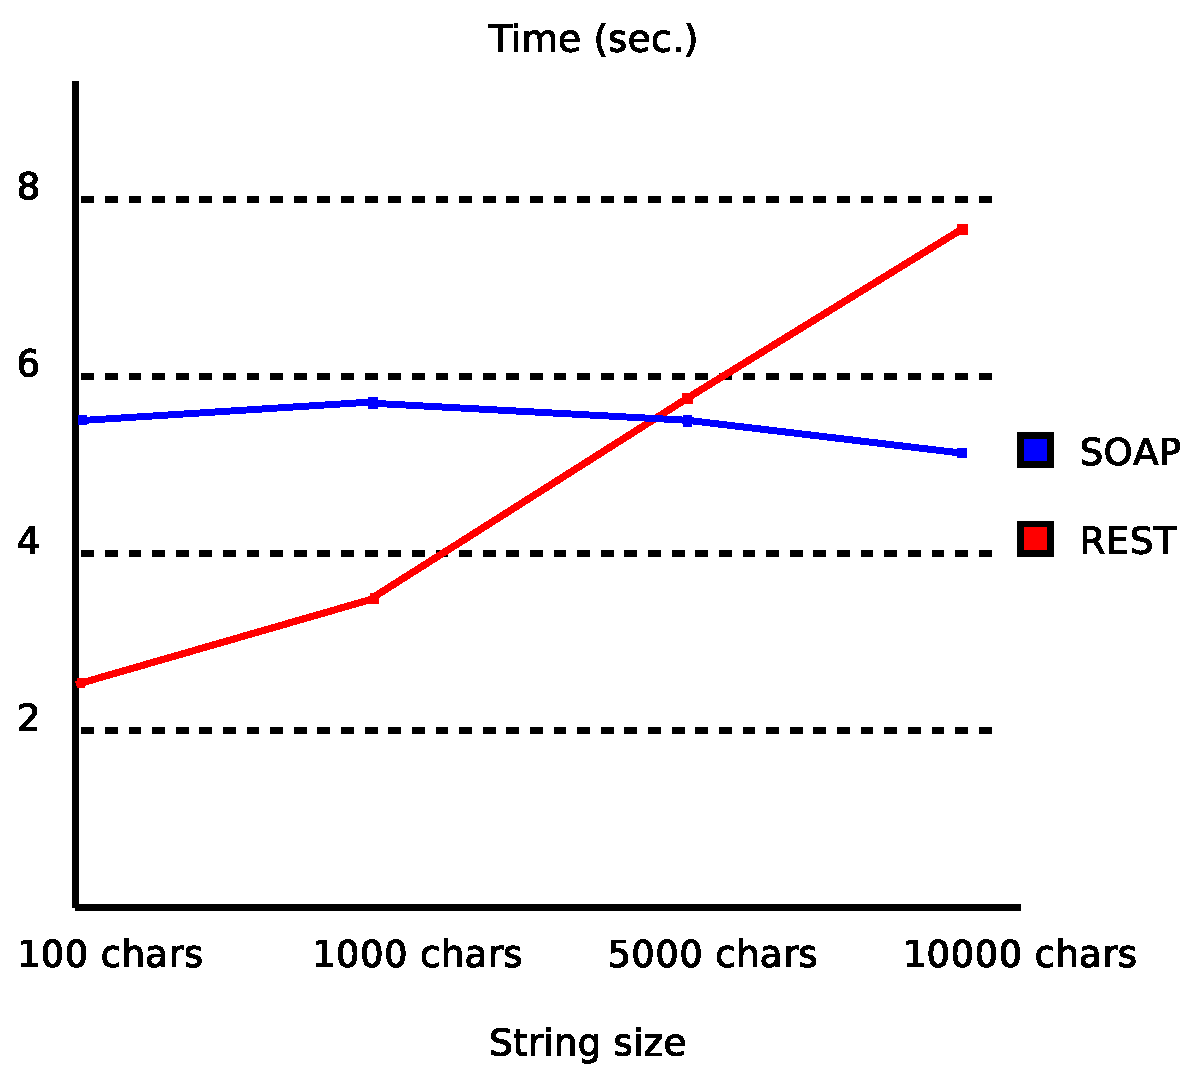
\epsfig{file=exp1.eps,width=8cm}
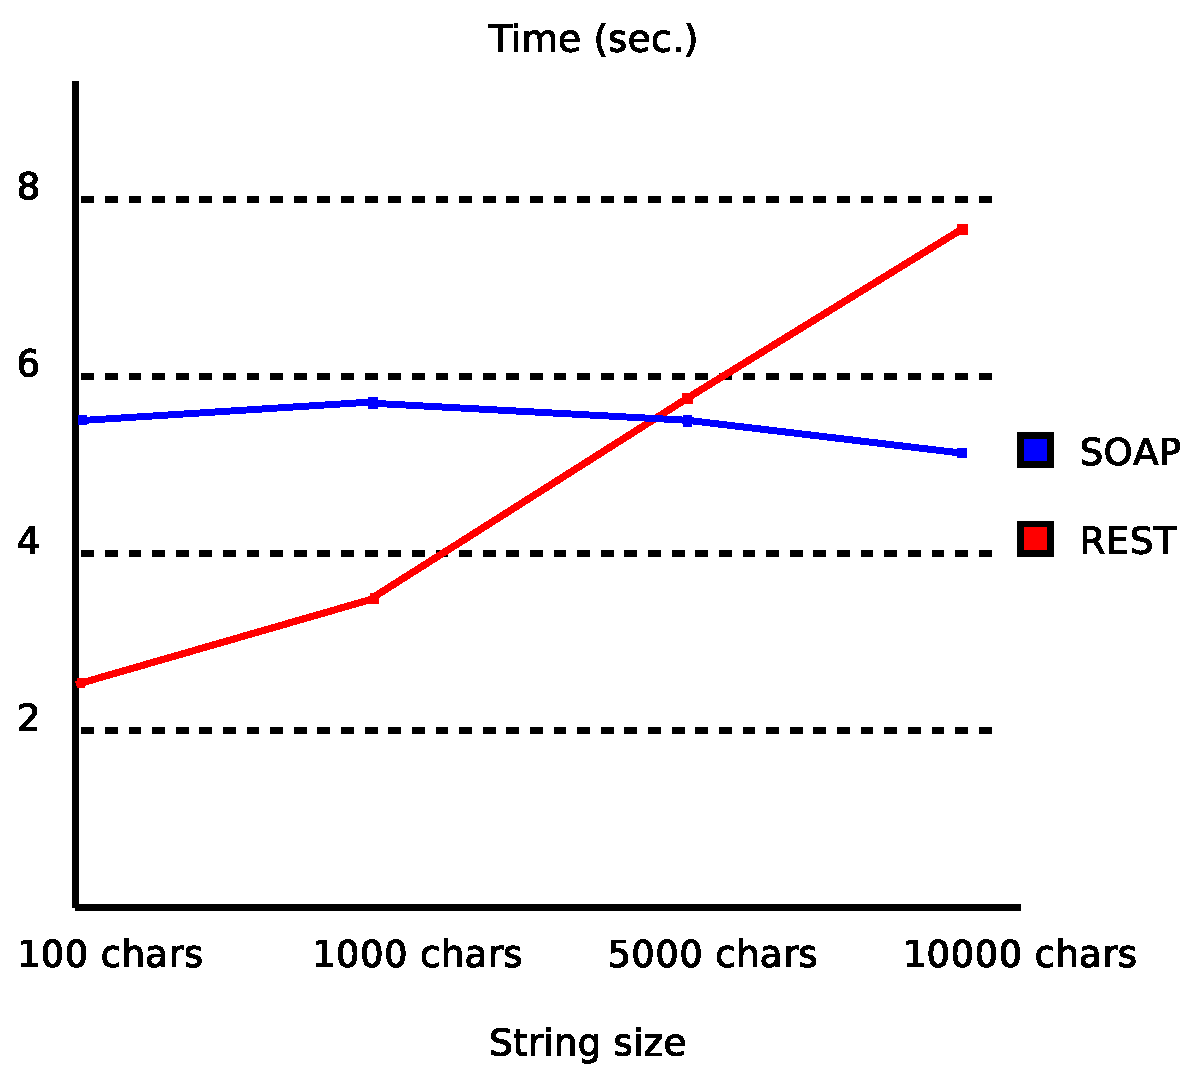
\includegraphics[width=8cm]{exp1.eps}
\caption{Time taken to complete the first experiment as the string size (amount of data) increases. About 5000 chars both implementations take a similar time.}
\label{figure:exp1}
\end{center}
\end{figure}

Results were verified using t-Student statistical tests and significant differences were found when the confidence level was $95\%$ or $99\%$. 

%-----------------------------------------------------------------------
\subsection{Master-Slave based GA Implementation}
\label{subsect:experiment2}

In the Experiment 2, we have parallelized a GA following a master-slave model in order to solve a function optimization problem.

As stated before, an ideal client-server implementation of a distributed evolutionary algorithm could be a server process with several threads, in which each thread would include a population.
However, as we cannot use a threaded version of the Perl modules, our implementation will focus on the fitness function evaluation.

Thus, the simplest way of task distribution along this model is to evaluate the individual fitness function on the slaves and to do the other steps on a master process ({\em farming}) as shown in Figure \ref{fig:esquema}.


\begin{figure}[!ht]
\begin{center}
%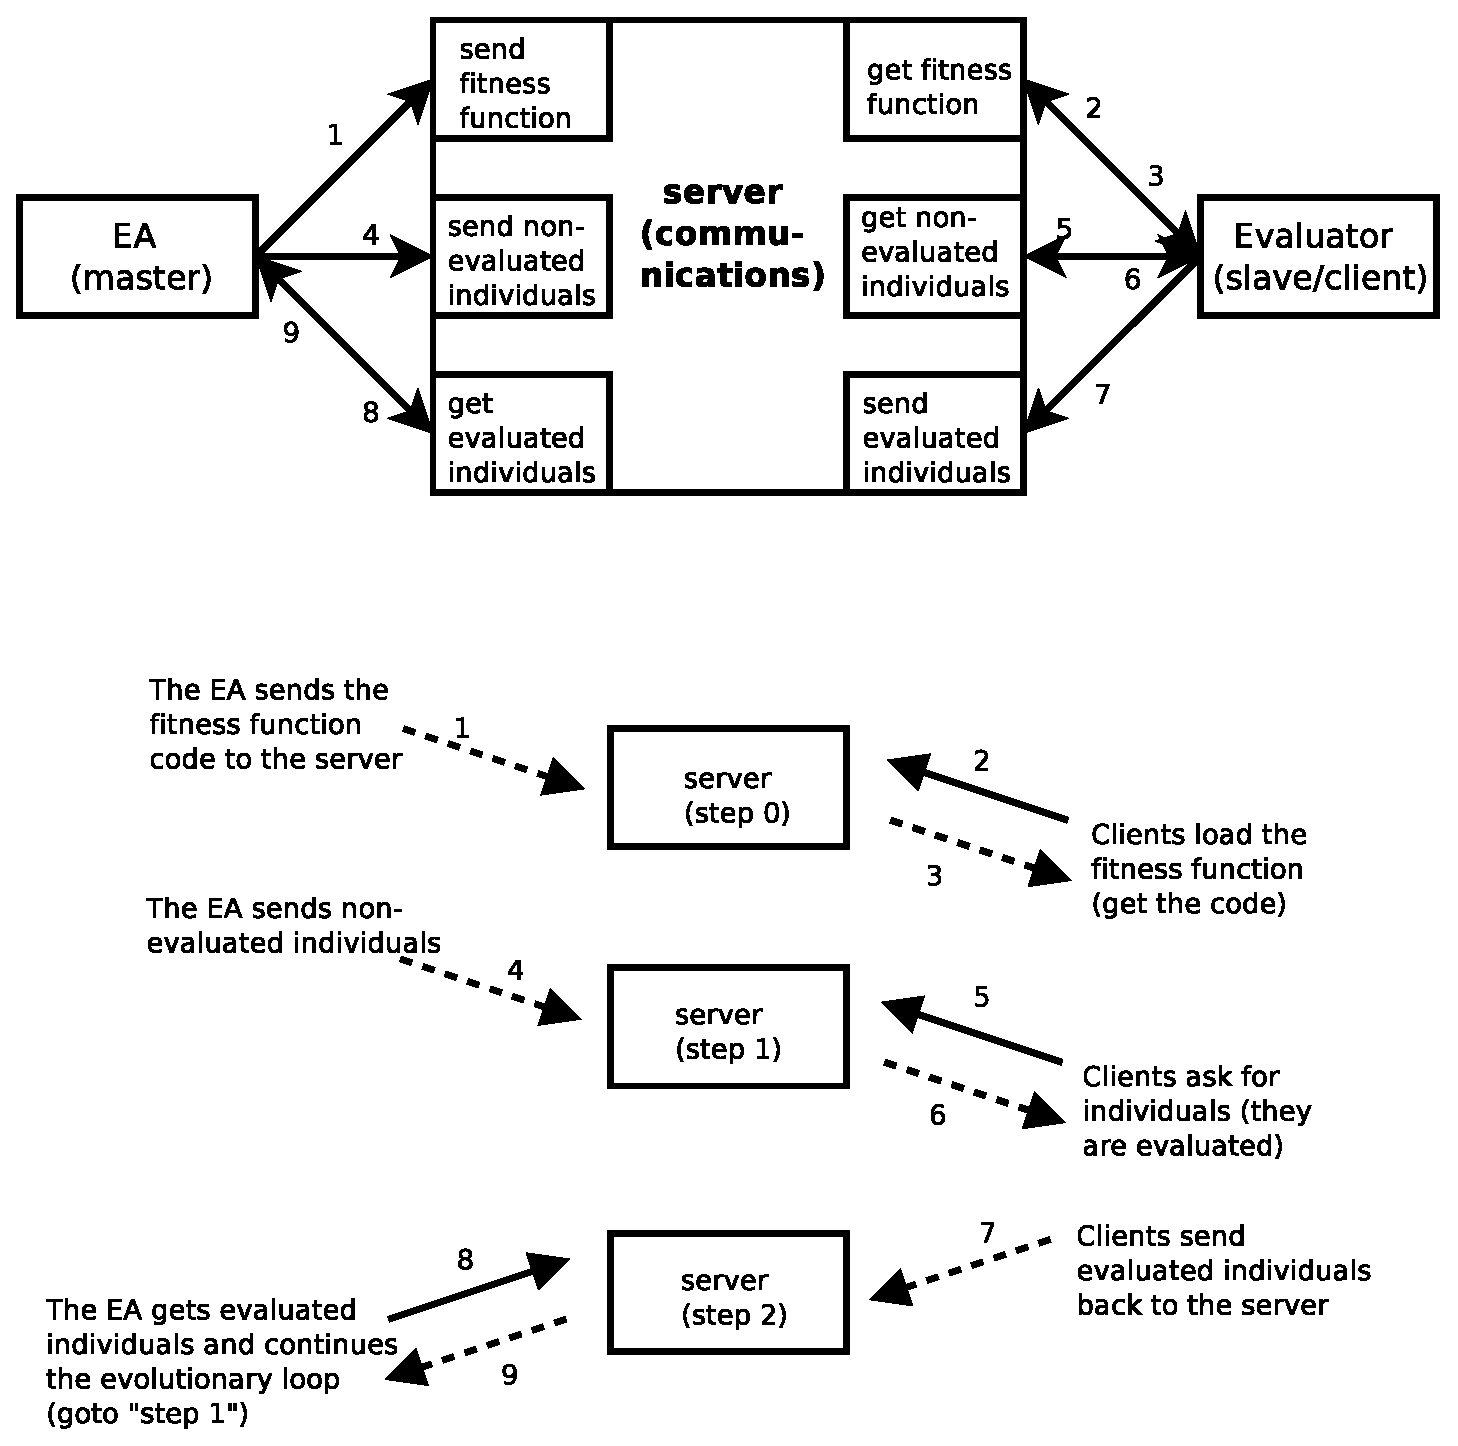
\epsfig{file=esquema.eps,width=9cm}
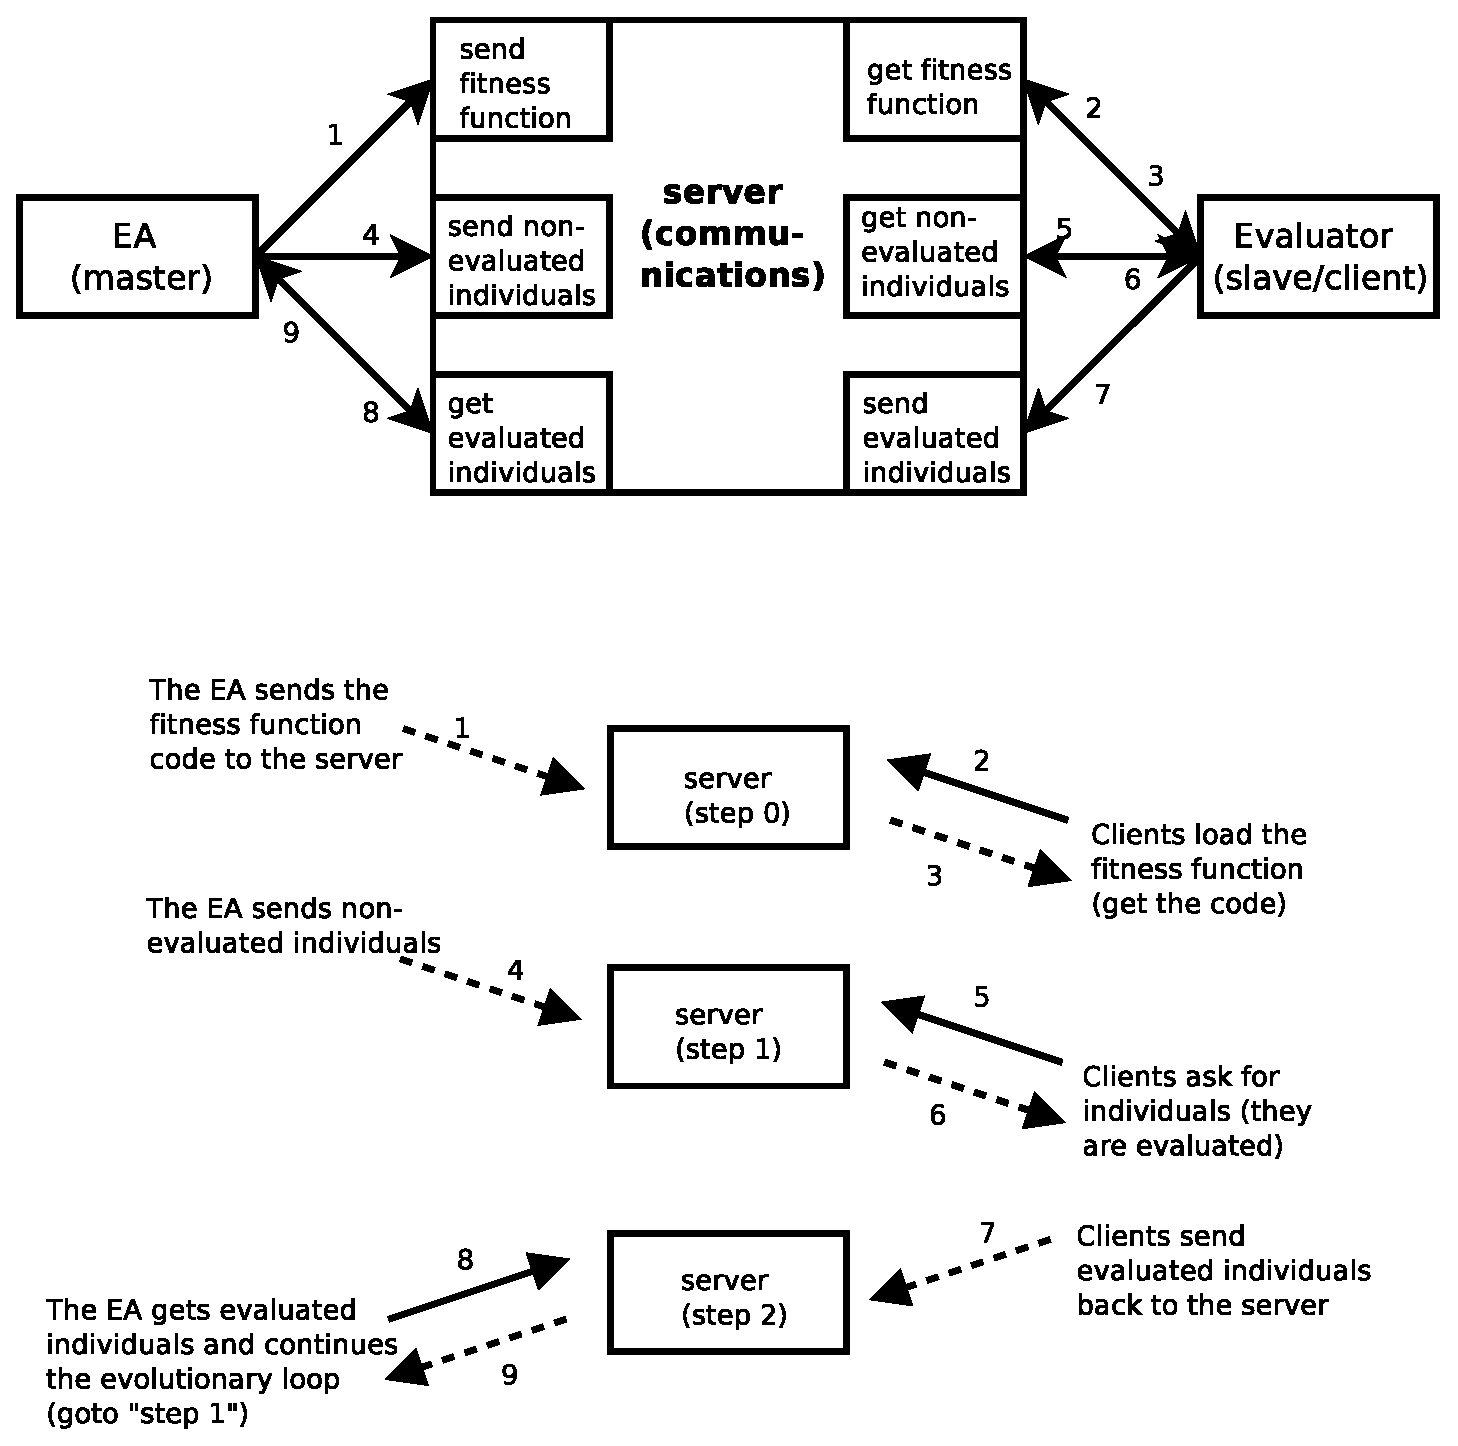
\includegraphics[width=8cm]{esquema.eps}
\caption{Schema of the master-slave based implementation. The master process runs the EA/GA and the slave processes evaluate the fitness function. The dotted lines represent data transfers from or to the server, while solid lines refer to requests to the server.} 
\label{fig:esquema}
\end{center}
\end{figure}


The evolutionary algorithm has been implemented using the A::E library
\cite{perl-ea},\cite{jjSOCO2010}, available under GPL
license\footnote{\url{http://opeal.sourceforge.net}}, in its version 0.76.2.

In this experiment, the fitness function is devoted to optimize the function given by equation \ref{ecu:Marea}, which is plotted in Figure \ref{fig:graficaMarea}. Our aim is to find the optimum ($f(0,0)=1$) with an accuracy of $10^{-6}$. 
The experiment was repeated for 30 times for each configuration, measuring the time spent using \emph{gettimeofday} function.

\begin{eqnarray}
f(x,y)=1+\frac{sin(\sqrt{x^{2}+y^{2}})}{\sqrt{x^{2}+y^{2}}} 
\label{ecu:Marea}
\end{eqnarray}

\begin{figure}[!ht]
\begin{center}
%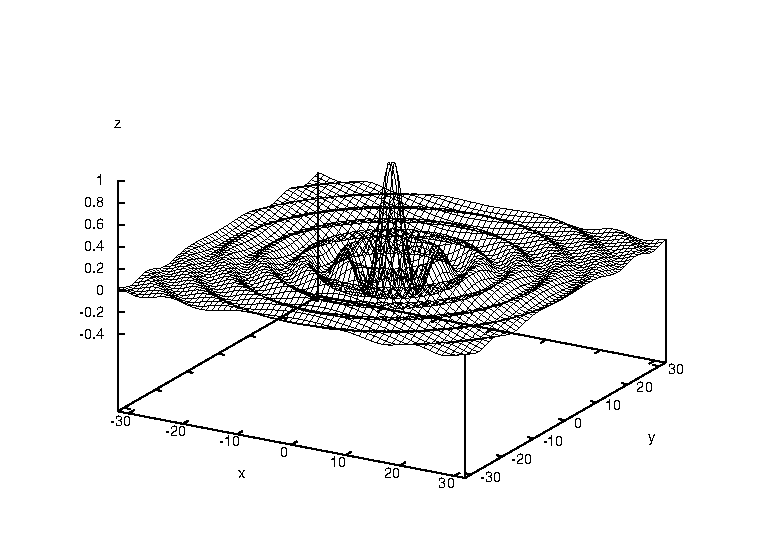
\epsfig{file=marea.eps,width=9cm}
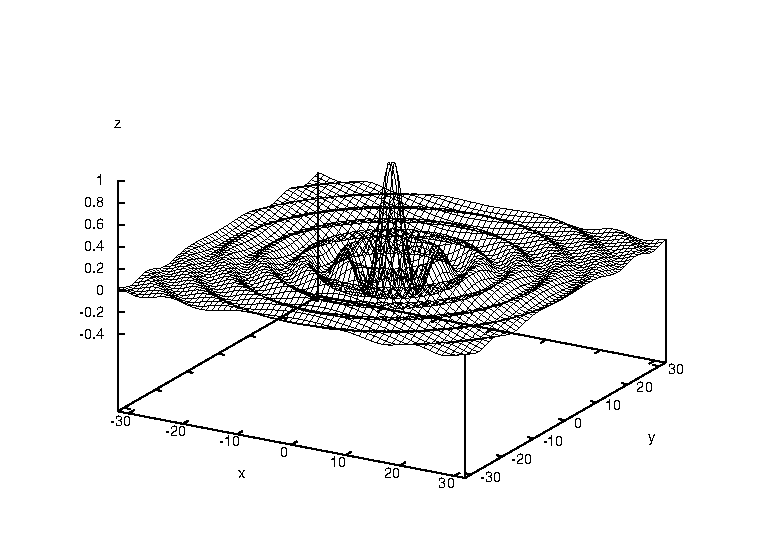
\includegraphics[width=9cm]{marea.eps}
\caption{Fitness function representation (given by equation \ref{ecu:Marea}). The optimum of this function is $f(0,0)=1$.}
\label{fig:graficaMarea}
\end{center}
\end{figure}

GA individuals are represented using bitstrings (data type {\sf A::E::Individual::BitString}). 
As genetic operators, a bitflip mutation ({\sf A::E::Op::Mutation}) and a two points crossover ({\sf A::E::Op::Crossover}) are used.

Remainder GA parameter values are set as follows (default values found after an intensive experimentation are used, since we do not intend to find the optimal ones, but to prove feasibility of the implementation, and carry out a comparison):

\begin{itemize}
   \item Population size = 50
   \item Generations = 20
   \item Individual length = 64 bits
   \item Mutation rate = $20\%$
   \item Crossover rate = $80\%$
   \item Selection rate = $40\%$
\end{itemize}


\begin{table*}[!ht]
\small{
\begin{tabular}{|l|r|l|l|l|l|}
\hline 
\multicolumn{2}{|c|}{}               &   10 generations        & 20 generations           & 50 generations           & 100 generations    \\
\multicolumn{2}{|c|}{}               &   10 individuals        & 50 individuals           & 50 individuals           & 100 individuals    \\
\hline
\ \ SOAP&accuracy     & \textbf{0.997942 $\pm$ 0.000762} * &\textbf{0.999867 $\pm$ 0.000101} *   &\textbf{1}                         &\textbf{1}    \\
             &time (sec.)  & 3.79 $\pm$ 0.42         &31.03 $\pm$ 1.89          &133.08 $\pm$ 0.91         &264.87 $\pm$ 0.39       \\
\hline
\ \ REST&accuracy     & 0.996092 $\pm$ 0.004081 &0.999976 $\pm$ 0.000003   &\textbf{1}                         &\textbf{1}     \\
             &time (sec.)  & \textbf{2.06 $\pm$ 0.08} *   &\textbf{15.05 $\pm$ 1.17} *          &\textbf{40.75 $\pm$ 2.81} *          &\textbf{100.84 $\pm$ 0.55} *       \\
\hline
\end{tabular}
}
\caption{Results obtained on the second experiment (master-slave implementations). The best results are highlighted in order to ease interpretation (asterisks indicate significant differences regarding the other results). 
%Both implementations obtain good results using even a small number of generations and population size. As far as the running time is concerned, REST implementation is faster in all configurations (10 gen./10 indiv. ; 20 gen./50 indiv. ; 50 gen./50 indiv. ; 100 gen./100 indiv.) as the message size is small.  
\label{tabla:exp2} }
\end{table*}


The  source code for all programs (servers, GA and evaluators), links
to the A::E library and experiment data are available for download
under GPL\footnote{\url{http://geneura.ugr.es/~pedro/research/webservices}}. % \ \ \ We would be grateful if this paper was referenced when using them in any research work}.

Table \ref{tabla:exp2} shows the results obtained for this function optimization problem.
The best results have been highlighted in order to ease interpretation, and asterisks have been used to indicate significative differences regarding the other results.
As can be seen, the REST implementation is faster, due to the SOAP verbosity and time taken to decode the XML messages.


Both implementations obtain good results in terms of accuracy (both find the optimum with an accuracy of $10^{-6}$) using even a small number of generations and population size. 
As far as the running time is concerned, REST implementation is faster in all configurations (see Table \ref{tabla:exp2} and Figure \ref{figure:exp2}). 
It might be due to the XML verboseness of SOAP communications (that increases the time taken to parse the messages).
This result was expected taking into account the results obtained in the first experiment (subsection \ref{subsect:experiment1}), as the message size in this experiment is small (64 chars). T-Student tests reported significant differences when the confidence level was $99\%$.

\begin{figure}[!ht]
\begin{center}
%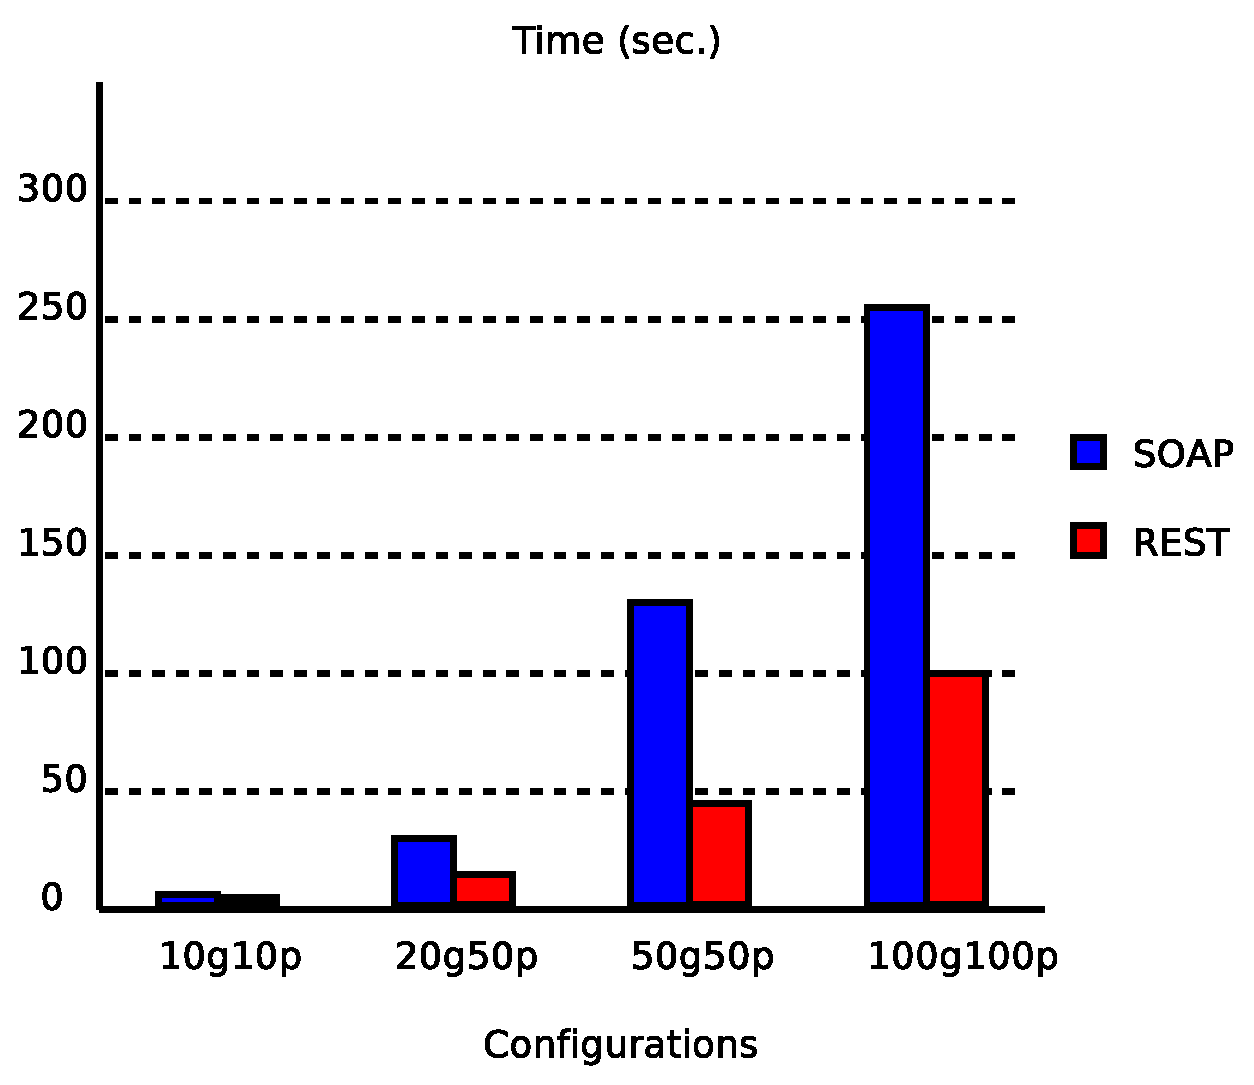
\epsfig{file=exp2.eps,width=8cm}
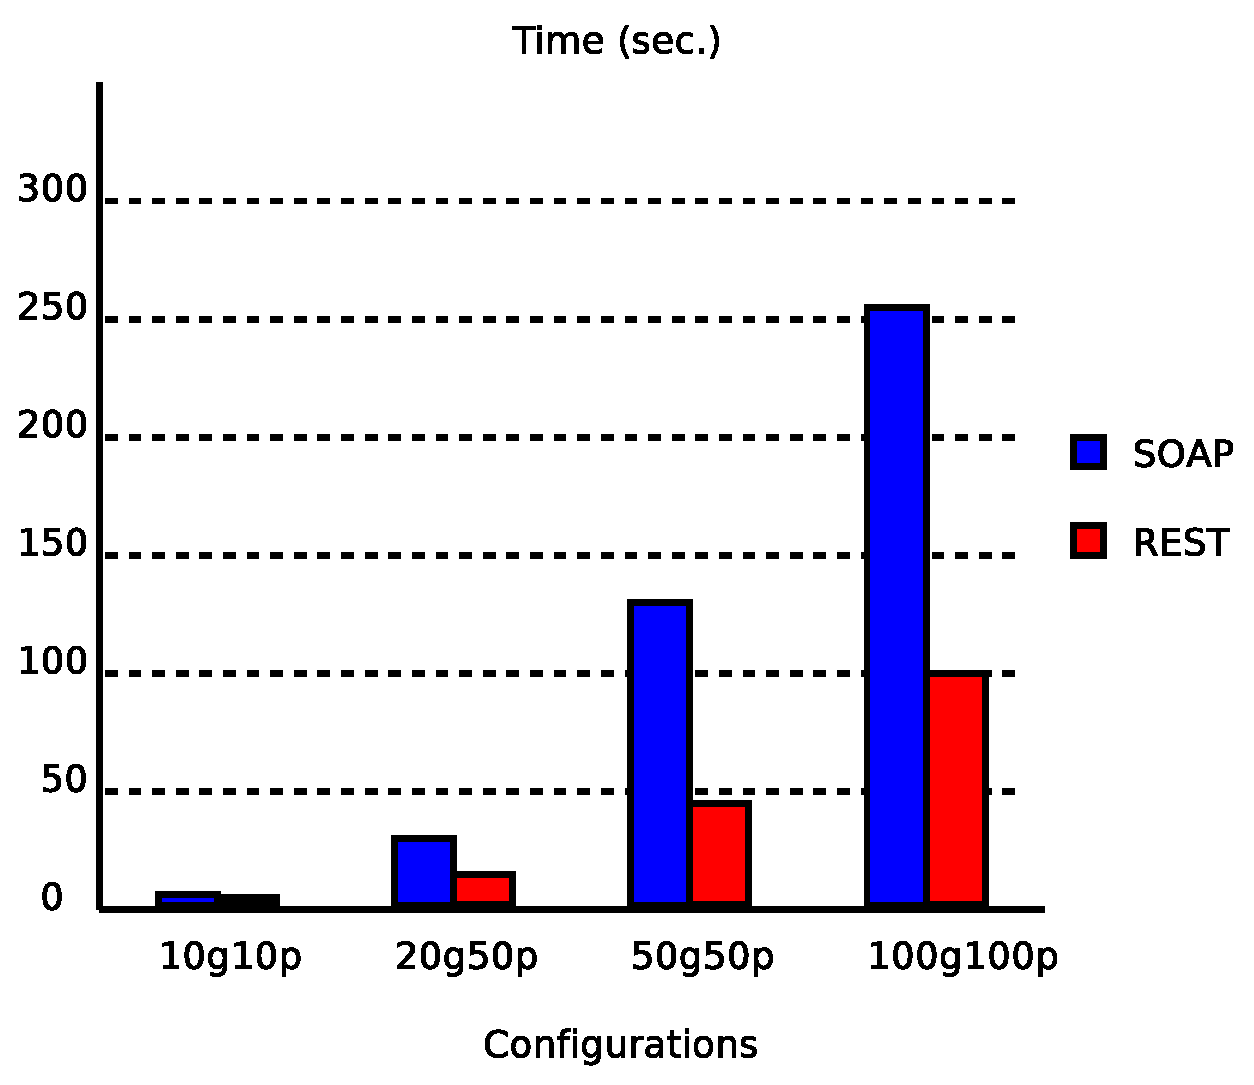
\includegraphics[width=8cm]{exp2.eps}
\caption{Comparing time (seconds) taken to complete the second experiment for each configuration (10 gen./10 indiv. ; 20 gen./50 indiv. ; 50 gen./50 indiv. ; 100 gen./100 indiv.). 
%As the message size is small, REST implementation yields better results as far as running time is concerned.
}
\label{figure:exp2}
\end{center}
\end{figure}

%REST implementation is faster due to the fact that no extra XML information is sent (that reduces the time taken to parse the messages).



%-----------------------------------------------------------------------
\subsection{Master-Slave based real coded EA Implementation}
\label{subsect:experimentREVIEW}

In this experiment, as in the previous one, we have parallelized an EA following a master-slave model in order to solve a function optimization problem using real coded individuals. 
%As in the previous experiment, the individual fitness is evaluated on the slaves, while the remainder steps are carried out on the master process. Both have been implemented using the A::E library.

In this case, three well known function approximation problems, taken from the CEC2005 Competition \cite{HansenCOMPETITION1}, are used: F7 Shifted Rotated Griewangk´s Function, F8 Shifted Rotated Ackley's Function and F9 Shifted Rastrigin's Function.
Detailed description of functions and conditions of testing are defined in \cite{HansenCOMPETITION2}, thus we provide only a brief information about the benchmark:

\begin{itemize}

%\item The Griewangk function \cite{GRIE81} is a continuous multimodal function with a high number of local optima. Its global optimum is located at $(0,...,0)$ \cite{DBLP:journals/amc/ChoOG08}. This problem has been used with vectors of 100 real numbers in the interval $[-512, 512]$.

\item The Griewangk function \cite{GRIE81} is a continuous multimodal function with a high number of local optima. It is defined according to Equation \ref{ecuacion:griewank} and its global optimum is located at point $x_{i}=0, i=1:Dimension$ (n real numbers in the interval $[0, 600]$) \cite{DBLP:journals/amc/ChoOG08}. 
\begin{equation}
 f_{n}(\vec{x}) = \frac{1}{4000} \sum_{i=1}^n x_{i}^2 - \prod_{i=1}^n cos \frac{x_{i}}{\sqrt{i}} + 1
\label{ecuacion:griewank}
\end{equation} 


\item The Ackley function \cite{funcs_ACK87,funcs_BAC96} (see Equation \ref{ecuacion:Ackley}) is a multimodal non separable and regular function usually used as test function. The global optimum is located at point $x_{i}=0, i=1:Dimension$ (n real numbers in the interval $[-32, 32]$).
\begin{equation}
f_{n}(\vec{x}) = 20+ e -20 \exp [-0.2\sqrt{\frac{1}{n} \sum_{i=1}^n x_{i}^2 } ]
\label{ecuacion:Ackley} 
\end{equation}

\begin{center}

$ - \exp [\frac{1}{n} \sum_{i=1}^n (cos(2 \pi x_{i})] $

\end{center}


%\item The Rastrigin function \cite{TZ89} is a multimodal real function optimization problem,  whose global optimum is located at point 0 and whose minimum value is 0. This problem has been addressed with vectors of 100 real numbers in the interval $[-512, 512]$.

\item The Rastrigin function \cite{TZ89} (see Equation \ref{ecuacion:rastrigin}) is a multimodal real function optimization problem,  whose global optimum is located at point $x_{i}=0, i=1:Dimension$ (n real numbers in the interval $[-50, 50]$) and whose minimum value is 0. 
\begin{equation}
 f_{n}(\vec{x}) = 10 n +\sum_{i=1}^n x_{i}^2 - 10 cos(2 \pi x_{i}) \\
\label{ecuacion:rastrigin}
\end{equation} 


\end{itemize}



\begin{table*}[!ht]

\scriptsize{
\begin{tabular}{|c|c|c||c|c||c|c|}
\hline 
\textbf{10D}& \multicolumn{2}{|c||}{F7} & \multicolumn{2}{|c||}{F8}    & \multicolumn{2}{|c|}{F9}    \\
\hline
       &\ \ \ \ \ \ \ \ \ \ Fitness\ \ \ \ \ \ \ \ \ \ &\ \ \ \ \ \ \ \ Time\ \ \ \ \ \ \ \ &\ \ \ \ \ \ \ \ \ \ Fitness\ \ \ \ \ \ \ \ \ \ &\ \ \ \ \ \ \ \ Time\ \ \ \ \ \ \ \ &\ \ \ \ \ \ \ \ \ \ \ \ Fitness\ \ \ \ \ \ \ \ \ \ \ \ &\ \ \ \ \ \ \ \ Time\ \ \ \ \ \ \ \  \\
\cline{2-7}
 SOAP  & 0.00015 $\pm$ 0.00014 &  495.39 $\pm$ 84.49 & \textbf{0.06561 $\pm$ 0.03905}*  & 429.23 $\pm$ 73.39 &  \ \ \textbf{7.05259 $\pm$ 4.42092} \ \ \ \ & 504.65 $\pm$ 74.21  \\
 REST  & \textbf{0.00015 $\pm$ 0.00012} \ \ &  \textbf{186.86 $\pm$ 45.34}* &  0.08998 $\pm$ 0.05155  & \textbf{115.83 $\pm$ 56.82}* &  7.28343 $\pm$ 5.30282 & \textbf{132.79 $\pm$ 64.13}*  \\
\hline
\end{tabular}
}
\scriptsize{
\begin{tabular}{|c|c|c||c|c||c|c|}
\hline 
\textbf{30D}& \multicolumn{2}{|c||}{F7} & \multicolumn{2}{|c||}{F8}    & \multicolumn{2}{|c|}{F9}    \\
\hline
       &\ \ \ \ \ \ \ \ \ \ Fitness\ \ \ \ \ \ \ \ \ \ &\ \ \ \ \ \ \ \ Time\ \ \ \ \ \ \ \ &\ \ \ \ \ \ \ \ \ \ Fitness\ \ \ \ \ \ \ \ \ \ &\ \ \ \ \ \ \ \ Time\ \ \ \ \ \ \ \ &\ \ \ \ \ \ \ \ \ \ \ \ Fitness\ \ \ \ \ \ \ \ \ \ \ \ &\ \ \ \ \ \ \ \ Time\ \ \ \ \ \ \ \  \\
\cline{2-7}
 SOAP  & \textbf{0.07914 $\pm$ 0.06043} \ \ &  530.44 $\pm$ 69.24 &  \textbf{0.08072 $\pm$ 0.09827} \ \  & 437.83 $\pm$ 54.82 &  \textbf{58.48678 $\pm$ 31.03845} \ \ & 510.96 $\pm$ 62.24  \\
 REST  & 0.08314 $\pm$ 0.05682 &  \textbf{192.82 $\pm$ 35.68}* &  0.10108 $\pm$ 0.12812  & \textbf{151.86 $\pm$ 38.06}* &  59.44189 $\pm$ 25.22289 & \textbf{130.19 $\pm$ 59.16}*  \\
\hline
\end{tabular}
}
\scriptsize{
\begin{tabular}{|c|c|c||c|c||c|c|}
\hline 
\textbf{50D}& \multicolumn{2}{|c||}{F7} & \multicolumn{2}{|c||}{F8}    & \multicolumn{2}{|c|}{F9}    \\
\hline
       &\ \ \ \ \ \ \ \ \ \ Fitness\ \ \ \ \ \ \ \ \ \ &\ \ \ \ \ \ \ \ Time\ \ \ \ \ \ \ \ &\ \ \ \ \ \ \ \ \ \ Fitness\ \ \ \ \ \ \ \ \ \ &\ \ \ \ \ \ \ \ Time\ \ \ \ \ \ \ \ &\ \ \ \ \ \ \ \ \ \ \ \ Fitness\ \ \ \ \ \ \ \ \ \ \ \ &\ \ \ \ \ \ \ \ Time\ \ \ \ \ \ \ \  \\
\cline{2-7}
 SOAP  & \textbf{1.08943 $\pm$ 0.63059}* &  523.58 $\pm$ 39.08 &  \textbf{0.19719 $\pm$ 0.16046} \ \  & 489.28 $\pm$ 85.38 &  \textbf{103.83096 $\pm$ 89.35315} & 516.61 $\pm$ 75.87  \\
 REST  & 1.46513 $\pm$ 0.90554 &  \textbf{198.37 $\pm$ 63.43}* &  0.20136 $\pm$ 0.17978  & \textbf{147.86 $\pm$ 53.04}* &  124.07184 $\pm$ 95.55851 & \textbf{152.57 $\pm$ 68.09}*  \\
\hline
\end{tabular}
}

\caption{Results obtained on the third experiment (master-slave implementations). The best results are highlighted in order to ease interpretation (asterisks indicate significant differences regarding the other results). 
%Both implementations obtain good results using even a small number of generations and population size. As far as the running time is concerned, REST implementation is faster as the message size is small.  
\label{tabla:expREVIEW} }

\end{table*}



These problem functions have been addressed for 10D, 30D and 50D, and, in all cases, as the optimum is known, the fitness of an individual is calculated as the distance to the optimum for that function, and the goal is to obtain the smallest fitness for the optimized function.

%The experiment was repeated for 30 times for each configuration, measuring the time spent using \emph{gettimeofday} function.

EA individuals are represented using real number vectors (data type {\sf A::E::Individual::Vector}). 
As genetic operators, a gaussian mutation ({\sf A::E::Op::GaussianMu- tation}) and a two points crossover ({\sf A::E::Op::VectorCros- sover}) are used.

Remainder EA parameter values are set as follows (default values found after an intensive experimentation are used, since we do not intend to find the optimal ones, but to prove feasibility of the implementation, and carry out a comparison):

\begin{itemize}
   \item Population size = 100
   \item Generations = 100
   \item Individual length = 10, 30 and 50 real numbers
   \item Mutation rate = $20\%$
   \item Crossover rate = $80\%$
   \item Selection rate = $40\%$
\end{itemize}

%The  source code for all programs (servers, GA and evaluators), links to the A::E library and experiment data are available for download under GPL\footnote{\url{http://atc.ugr.es/pedro/research/webservices}}.

Table \ref{tabla:expREVIEW} shows obtained results for these function optimization problems.
The mean value and standard deviation of the fitness function are reported, as well as the time taken to run the algorithms.
The best results have been highlighted in order to ease interpretation, and asterisks have been used to indicate significative differences regarding the other results.
As can be seen, the REST implementation is faster, due to the SOAP verbosity and time taken to decode the XML messages.

Both implementations obtain good results in terms of accuracy (both achieve results close to the optimum) using even a small number of generations and population size. 
As far as the running time is concerned, REST implementation is faster due to the fact that no extra XML information is sent (that reduces the time taken to parse the messages) (see Table \ref{tabla:expREVIEW}). 
This result was expected taking into account the results obtained in the first experiment (subsection \ref{subsect:experiment1}), as the message size in this experiment is small, even for Dimension=50. T-Student tests reported significant differences when the confidence level was $99\%$.


As far as the convergence is concerned, Figure \ref{figure:expREVIEW} shows the fitness evolution for both Griewangk, Rastrigin and Ackley (using as dimension 10, 30 and 50). 
In some cases premature convergence can be observed.
This is due to the fact that no specific algorithm, selector nor genetic operators have been used to solve these problems (a canonical EA has been used).
%  La convergencia se estanca hacia la mitad. Esto se debe a que no usamos un algoritmo específico para este tipo de problemas, sino un canónico

\begin{figure*}[!ht]
\begin{center}
\setlength{\tabcolsep}{2mm}
\renewcommand{\arraystretch}{1.2}
\begin{tabular}{ccc}

 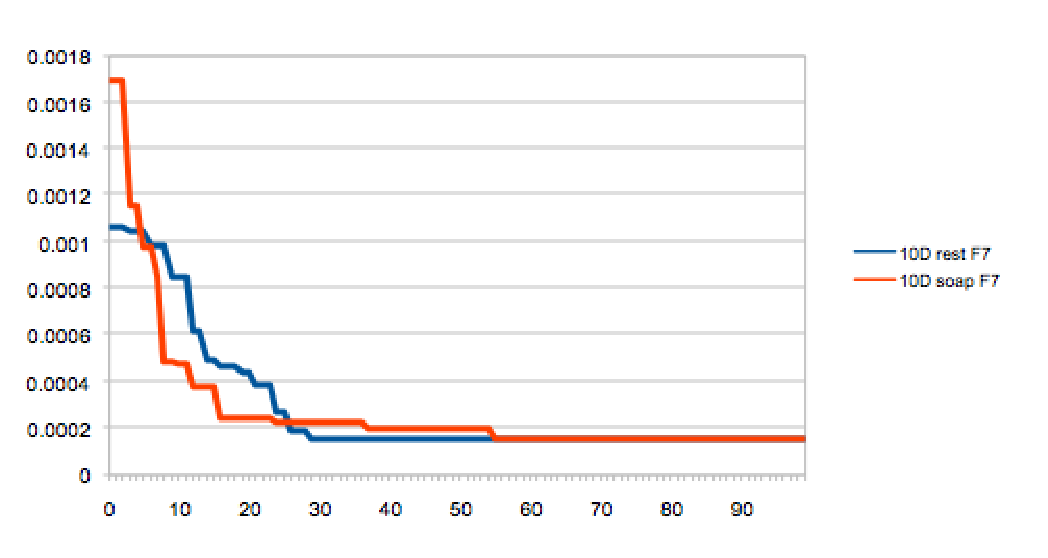
\includegraphics[width=5cm]{f7d10.eps}  & 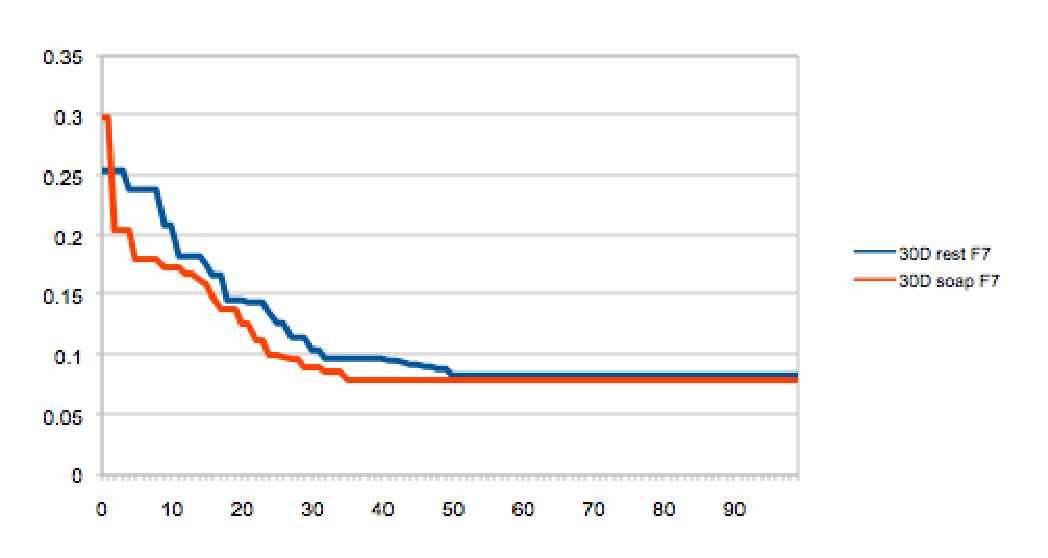
\includegraphics[width=5cm]{f7d30.eps}  &  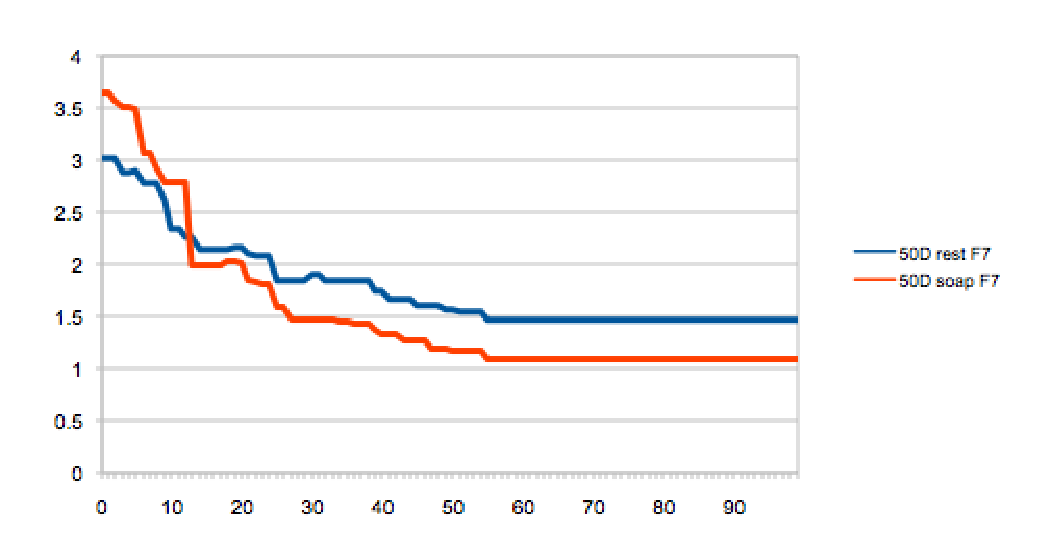
\includegraphics[width=5cm]{f7d50.eps}  \\
 
 F7 - 10D & F7 - 30D & F7 - 50D \\

 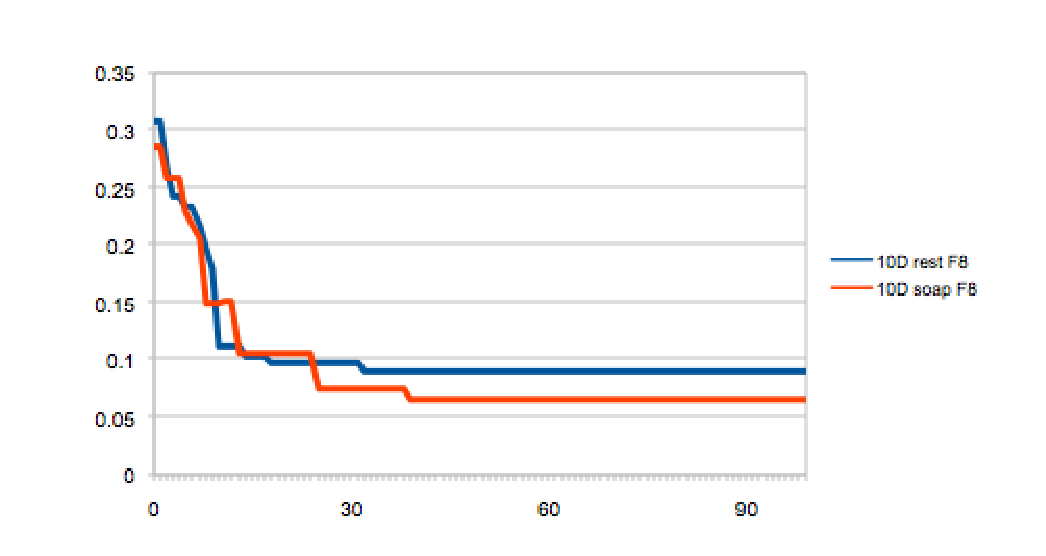
\includegraphics[width=5cm]{f8d10.eps}  & 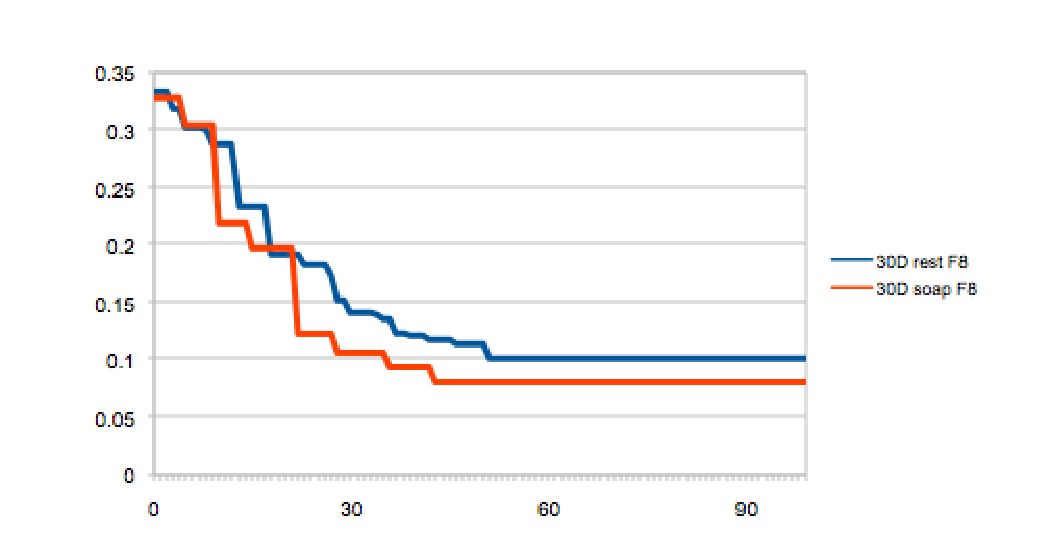
\includegraphics[width=5cm]{f8d30.eps}  &  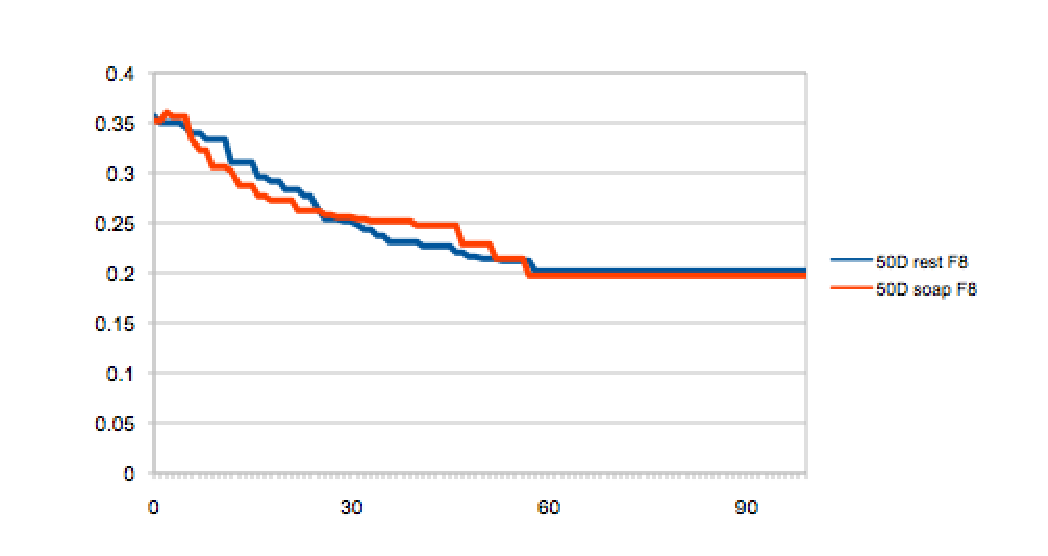
\includegraphics[width=5cm]{f8d50.eps}  \\
 
 F8 - 10D & F8 - 30D & F8 - 50D \\
 
 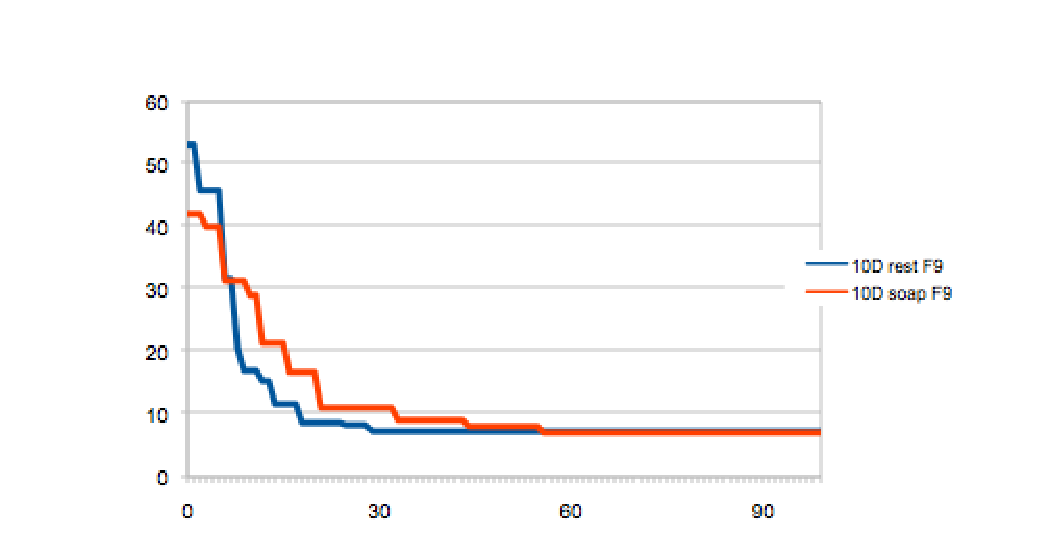
\includegraphics[width=5cm]{f9d10.eps}  & 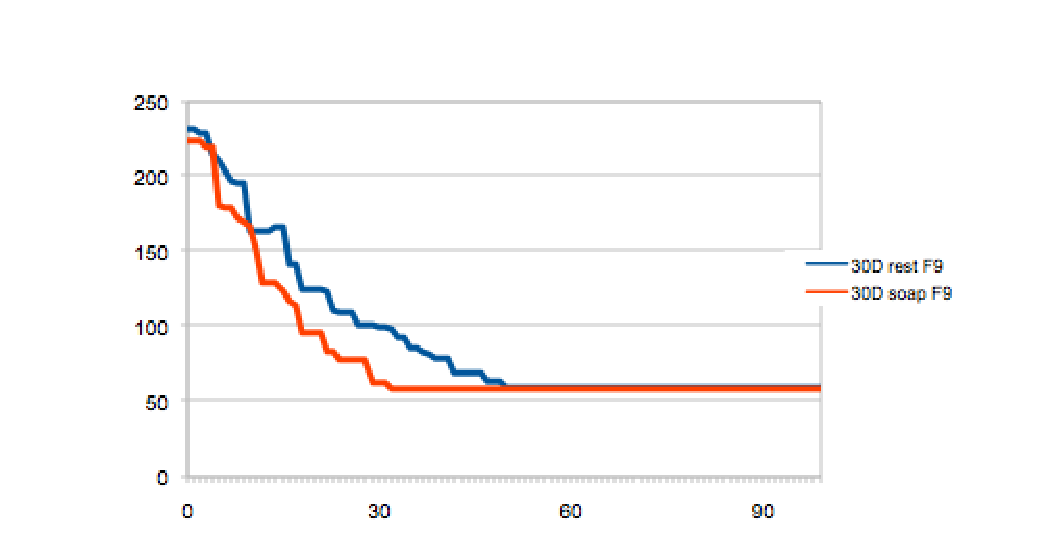
\includegraphics[width=5cm]{f9d30.eps}  &  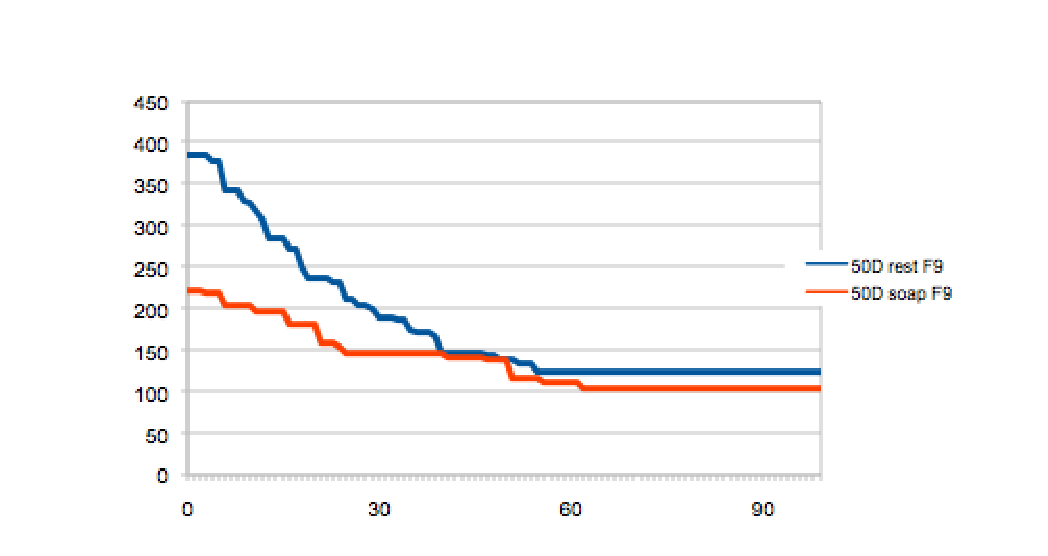
\includegraphics[width=5cm]{f9d50.eps}  \\
 
 F9 - 10D & F9 - 30D & F9 - 50D \\
 
\end{tabular}
\caption{Evolution of fitness for the three functions and different configurations (10D, 30D and 50D). Each figure compares best fitness in each generation, for both SOAP and REST implementations. }
\label{figure:expREVIEW}
\end{center}
\end{figure*}



The aim of this experiment is to use a costly and standard problem, focusing on comparing the performance of SOAP and REST implementations.
In any case, good results have been obtained using both approaches, even comparable to those that can be found in the bibliography \cite{Song2007,Fan2010,Qin2009}.




%-----------------------------------------------------------------------
\subsection{Master-Slave based EA implementation using Web-Services}
\label{subsect:experiment3}

In this experiment we adapt G-Prop as a distributed EA using SOAP and REST. Our implementation will focus on the most time consuming operation: the fitness function evaluation.
G-Prop leverages the capabilities of two classes of algorithms: the ability of EA to find a solution close to the global optimum, and the ability of the back-propagation algorithm (BP) to tune a solution and reach the nearest local minimum by means of local search from the solution found by the EA. 
G-Prop method has been fully described and analysed out in previous papers (see \cite{CastilloNPL},\cite{castilloNC}), thus we refer to these papers for further details.
Instead of using a pre-established topology, the population is initialised with different hidden layer sizes.
In most cases, evolved MLP should be coded into chromosomes to be handled by the genetic operators, however, G-Prop uses no binary codification, instead, the initial parameters of the network are evolved using specific variation operators such as mutation, multi-point crossover, addition and elimination of hidden units, and QP training applied as operator to the individuals of the population.
The EA optimises the classification ability of the MLP, and at the same time it searches for the number of hidden units (architecture), the initial weight setting and the learning rate for that net.


%The evaluation of the objective function is the most time consuming part in G-Prop. 
The whole evolutionary algorithm is run on a master process and only the objective function is sent to the slaves for evaluation, following a {\em farming} model (as shown in Figure \ref{fig:esquema}).

The whole system can be sketched as follows:
\begin{enumerate}
  \item The EA process sends the fitness function code to the server and creates the EA population.
  \item Some clients connect the server and load the fitness function sent as Perl code from the server (Figure \ref{fig:ejemploREST} shows an example of server and client processes implementations to upload and download the fitness function source code).
  \item The EA process sends non-evaluated individuals to the server.
  \item The clients ask for individuals to the server in order to evaluate them.
  \item The clients evaluate individuals and send the result back to the server.
  \item The EA process obtains evaluated individuals from the server and continues the evolutionary loop.
  \item The EA terminates after a fixed number of generations (it sends a termination message throughout the server to the clients that remain ready to attend new workloads).
\end{enumerate}


The server in these experiments is mainly used for scheduling and balancing the tasks among the different clients; the network itself is used for communication, but all the interchange of information among clients must be cleared by the central server. However, one of the objectives of the work presented in this paper has been to create an infrastructure that would get rid of the bottleneck represented by the central server in these experiments.
As in the previous experiments, the EA has been implemented using the A::E library.

%Again, the full source code (servers, EA and evaluators), links to the A::E library and experiment data are available under GPL\footnote{\url{http://atc.ugr.es/pedro/research/webservices}}.



%--------------------------------------------
\subsubsection{The experiment}

The tests used to assess the accuracy (obtained error) of a method must be carefully selected, since some synthetic problems (also called ``toy problems'') are not suitable for certain capacities of the BP algorithm, such as generalization \cite{FahlmanBENCHMARKS}. 
We agree with the view put forward by Prechelt \cite{Prechelt94c}, stating that real problems should be used in order to test an algorithm.
In real life problems, the division between classes is not as clear as it is in synthetic problems. The dispersion of samples within a single class is also greater, due to noise \cite{merelo:ESNN}. 
In any case, the best way to test the algorithm ability as well as its limitations is to use it to resolve real world problems.

In this paper, the Glass pattern classification problem is used.
This problem was put forward by Prechelt in his paper \emph{``{PROBEN1 -- A Set of Benchmarks and Benchmarking Rules for Neural Network Training Algorithms}''} \cite{Prechelt94c}.

This dataset is based on the glass problem dataset from the UCI library of machine learning databases.
This task was prompted by the needs of forensic scientists involved in criminal investigation.
The results of a chemical analysis of glass splinters (content of 8 different elements in percentage terms) together with a refractive index, are used in the classification of the sample as either float-processed or non-float processed building windows, vehicle windows, containers, tableware or head lamps. 
It contains 214 entries. Each sample has 9 attributes plus the class attribute (type of glass): refractive index, sodium, magnesium, aluminium, silicon, potassium, calcium, barium, and iron.
This dataset is very difficult to classify due to two important features. First, the number of available patterns is low (214) for six different classes. Second, the number of patterns in each class is very unbalanced, ranging from 76 (building windows non-float processed) to 9 (tableware).


Dataset was divided into three disjoint parts: one for training, one for validating, and one for testing, as proposed in \cite{Prechelt94c}. 
In order to determine the fitness of an individual, the MLP was trained by the training set and its fitness was established from the classification error with the validating set.
After the EA has finished, i.e. when it has reached the limit of generations, we obtain the generalization ability by using the testing set (previously unseen patterns). This generalization value is shown in tables.


\begin{table}[!h]
\small{
\begin{tabular}{|c|c|}
\hline 
Parameter & Value \\
\hline
\hline
\hline
number of generations   & 500 \\
\hline
population size & 500 \\
\hline
selection rate  & $20\%$ \\
\hline
initial weights range  & $[-0.05,0.05]$ \\
\hline
\hline
mutation operator priority        & 2.0   \\
\hline
crossover operator priority             & 0.5 \\
\hline
addition operator priority & 1.0   \\
\hline
elimination operator priority     & 0.5   \\
\hline
training operator priority     & 0.5   \\
\hline
\hline

mutation probability     & $0.4$   \\
\hline
weight mutation range     & $[-0.001,0.001]$   \\
\hline
learning constant mutation range     & $[-0.010,0.010]$   \\

%\hline
%\hline
%number of training epochs & 500 \\

\hline
\end{tabular}
}
\caption{Parameters set using statistical methods (see \cite{CastilloIEEETNN} for details). The number of generations and the population size needed for greater diversity should, of course, be higher or lower depending on the difficulty of the problem.  \label{tabla:parametros} }
\end{table}


On the other hand, it is very important to know which parameter values involved in the design of an EA have the greatest influence on its behaviour and performance.
%Traditionally, genetic algorithm users adjusted the main design parameters of an EA (crossover probability, mutation probability, population size, number of generations, selection rate) by hand \cite{Davis91}, \cite{Jagielska99},\cite{Das2009}. The decision on which values are optimal was usually made in terms of the most common values or experimental formulae given in the bibliography, or by trial and error \cite{Grefenstette86}, \cite{DKim97}. 
Adjusting the main design parameters has been usually solved either by hand \cite{Davis91}, \cite{Jagielska99},\cite{Das2009} or using conventions, ad-hoc choices, intensive experimentation with different values \cite{emss2007,smiteiben_paper_2009,eiben_tut_cec2009,smiteiben_paper_cec2009,SmitCEC2010}, and even random initialization values \cite{GongCEC2011}. As Eiben states, the straightforward approach is to generate and test \cite{DKim97,eiben_tut_cec2009,smiteiben_paper_cec2009}.
Nevertheless, when making a detailed statistical analysis of the influence of each parameter, the designer should pay greater attention to the parameter providing the values that are statistically most significant \cite{castillo2011}.

Authors carried out a statistical study \cite{CastilloIEEETNN} in order to determine the most important parameters (regarding their influence on the results), and to establish the most suitable values for such parameters (thus obtaining an optimal operation). In this study, the ANOVA (ANalysis Of the VAriance) \cite{Fisher25},\cite{Fisher36} statistical method was used. This statistical tool, based on the analysis of the mean variance, is widely used.
The ANOVA method was used to determine whether a change in the responses is due to a change in a factor or due to a random effect. Besides the ANOVA method, the statistical analysis tool ANOM (ANalysis Of Mean) was used. This technique uses the average values for each parameter level (value) and the main effect (on the responses) plots, to decide the most suitable values for each parameter. 
As a result, running parameter values shown in Table \ref{tabla:parametros} were obtained.

The number of generations and the population size needed for greater diversity should, of course, be higher or lower depending on the difficulty of the problem.

% sitio natural de la tabla de parametros obtenida con anova

Time taken to run the EA was measured using the \emph{gettimeofday} function, in order to achieve a good precision, from which mean and standard deviations (for 30 runs) shown in Table \ref{tabla:resultados3} were obtained.
%Time taken to run the EA is reported in Table \ref{tabla:resultados3}.
Sequential version of the program was run in the faster machine; and in parallel runs, 
the EA (master process) was run on the faster machine while the evaluators were run on slower machines.


% Statistical \emph{t-Student} tests are used to evaluate obtained results and to test whether differences among means are significant.


\subsubsection{Obtained Results}

%In this experiment we are not interested on comparing results against other authors, but in using a costly problem that justifies using a farming model.
The aim of this experiment  is to use a costly problem that justifies
using a farming model, but always with an emphasis on comparing the performance of SOAP and REST implementations.
Results obtained can be shown in Table \ref{tabla:resultados3}.
The best results have been highlighted in order to ease interpretation. In some cases, asterisks have been used to indicate significative differences regarding the other results.

\begin{table}[!h]
\small{
\begin{tabular}{|c|c|c|c|}
\hline 
Model         &  Error ($\%$)  &  Time (seconds)  \\
\hline
\hline
Sequential    &   33 $\pm$ 2   &   \textbf{1215 $\pm$ 104} *  \\    
\hline
\hline
\multicolumn{3}{|l|}{Master-slave (using SOAP)} \\
\hline
\ \ \ 1 eval. &   32.8 $\pm$ 1.3   &    1343 $\pm$ 116  \\
\hline
\ \ \ 2 eval. &   \textbf{32.2 $\pm$ 1.5}   &    \textbf{717 $\pm$ 81} *  \\
\hline
\ \ \ 3 eval. &   31.8 $\pm$ 1.3   &    \textbf{508 $\pm$ 91} *  \\
\hline
\ \ \ 4 eval. &   \textbf{31.0 $\pm$ 1.6} * &    \textbf{404 $\pm$ 89} *  \\
\hline
\hline
\multicolumn{3}{|l|}{Master-slave (using REST)} \\
\hline
\ \ \ 1 eval. &   \textbf{32.2 $\pm$ 1.6} * &    1517 $\pm$ 109  \\
\hline
\ \ \ 2 eval. &   32.4 $\pm$ 1.5   &    804 $\pm$ 89   \\
\hline
\ \ \ 3 eval. &   \textbf{31.4 $\pm$ 2.1}   &    566 $\pm$ 97   \\
\hline
\ \ \ 4 eval. &   31.6 $\pm$ 1.8   &    447 $\pm$ 82   \\
\hline
\hline
\end{tabular}
}
\caption{Results (error $\%$ and time) obtained using both the sequential and the parallel versions (comparing using the same number of evaluations). Up to 4 evaluators-slaves are used in the farming model. The best results are highlighted in order to ease interpretation (asterisks indicate significant differences regarding the other results). 
%Comparable classification ability is obtained; however, better results in time are obtained as the number of evaluators is increased (parallelizing the problem between several computers).  
\label{tabla:resultados3} }
\end{table}



\begin{figure}[!ht]
\begin{center}
%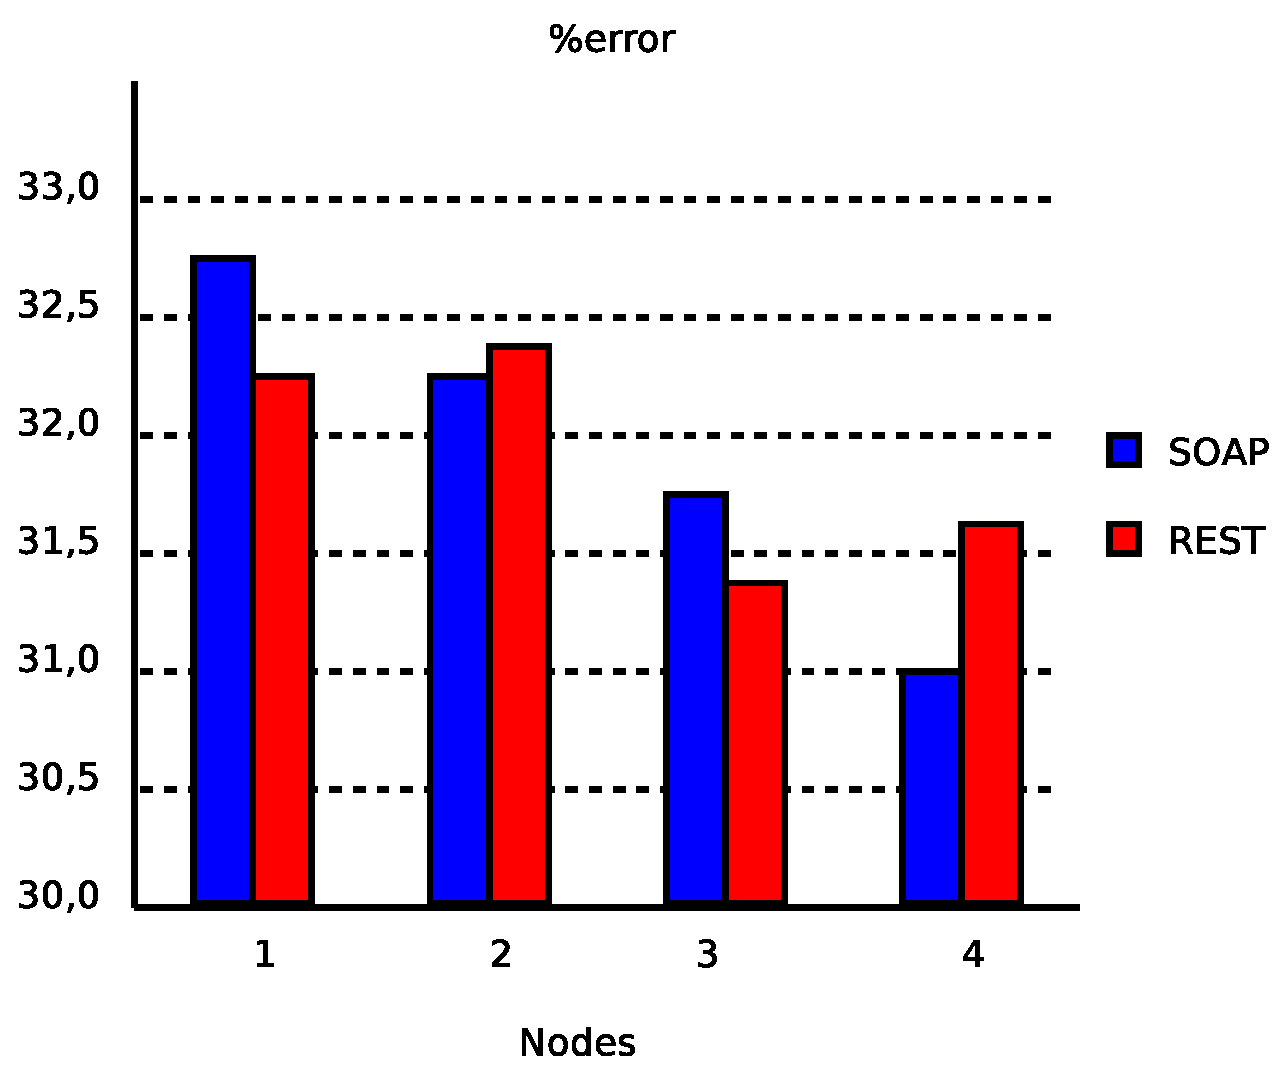
\epsfig{file=exp3_error.eps,width=8cm}
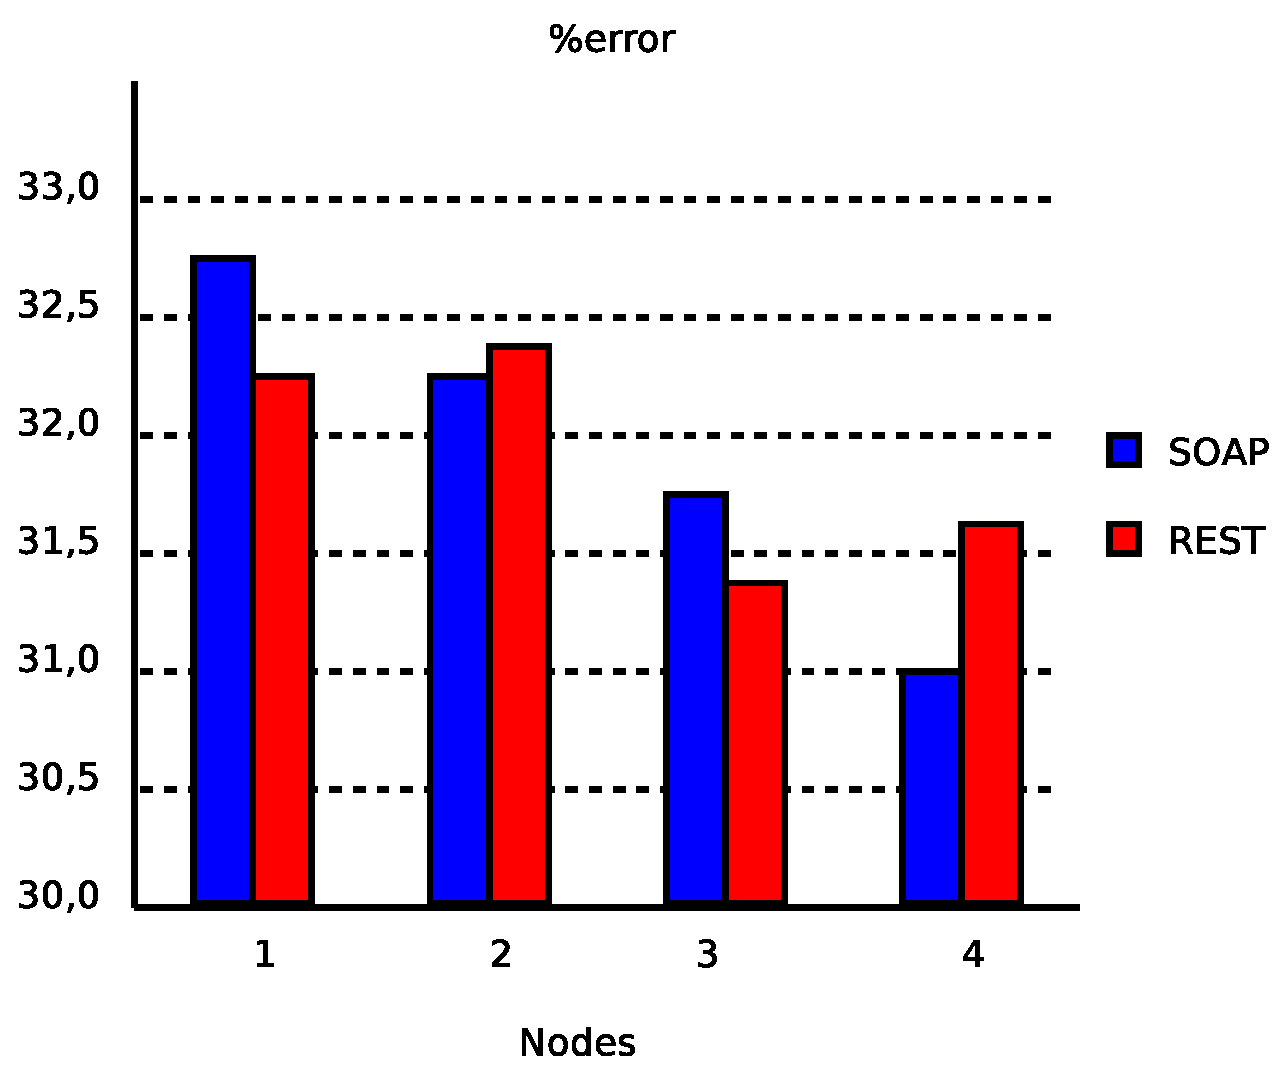
\includegraphics[width=8cm]{exp3_error.eps}
\caption{Plot of the classification error ($\%$). As can be seen, the results in error are very similar, what means that both techniques are suitable for developing parallel systems.}
\label{fig:resultados3error}
\end{center}
\end{figure}


Table \ref{tabla:resultados3} and Figure \ref{fig:resultados3error} show the generalization performance on previously unseen patterns, as well as the running time.
%Results shown in tables are obtained as the mean and standard deviation and the best results have been highlighted in order to ease interpretation.
As can be seen, classification errors show a comparable algorithmic result, as there are small differences on obtained error, although running time reduces when dividing the problem between several computers that work in parallel. 

Results were verified using t-Student statistical tests. 
In the case of classification error, significant differences were found when the confidence level was $80\%$. 
In some cases, the means were so similar that no significant differences were found (using 2 and 3 evaluators). 
In all cases, the resultant times presented significant differences when the confidence level was $95\%$ (using 3 and 4 evaluators) and even as high as $99\%$ for 1 and 2 evaluators. Note that the sequential model achieves a lower time, due to the fact that no communication overload is introduced in this case.

As can be seen in Figure \ref{fig:resultados3time}, SOAP implementation is slightly faster than the REST one, as the amount of data sent in each communication is very high (more than 6000 chars on average). This result is in agreement with the first experiment, where for large amounts of data (big messages), REST communications take longer than SOAP communications.


\begin{figure}[!ht]
\begin{center}
%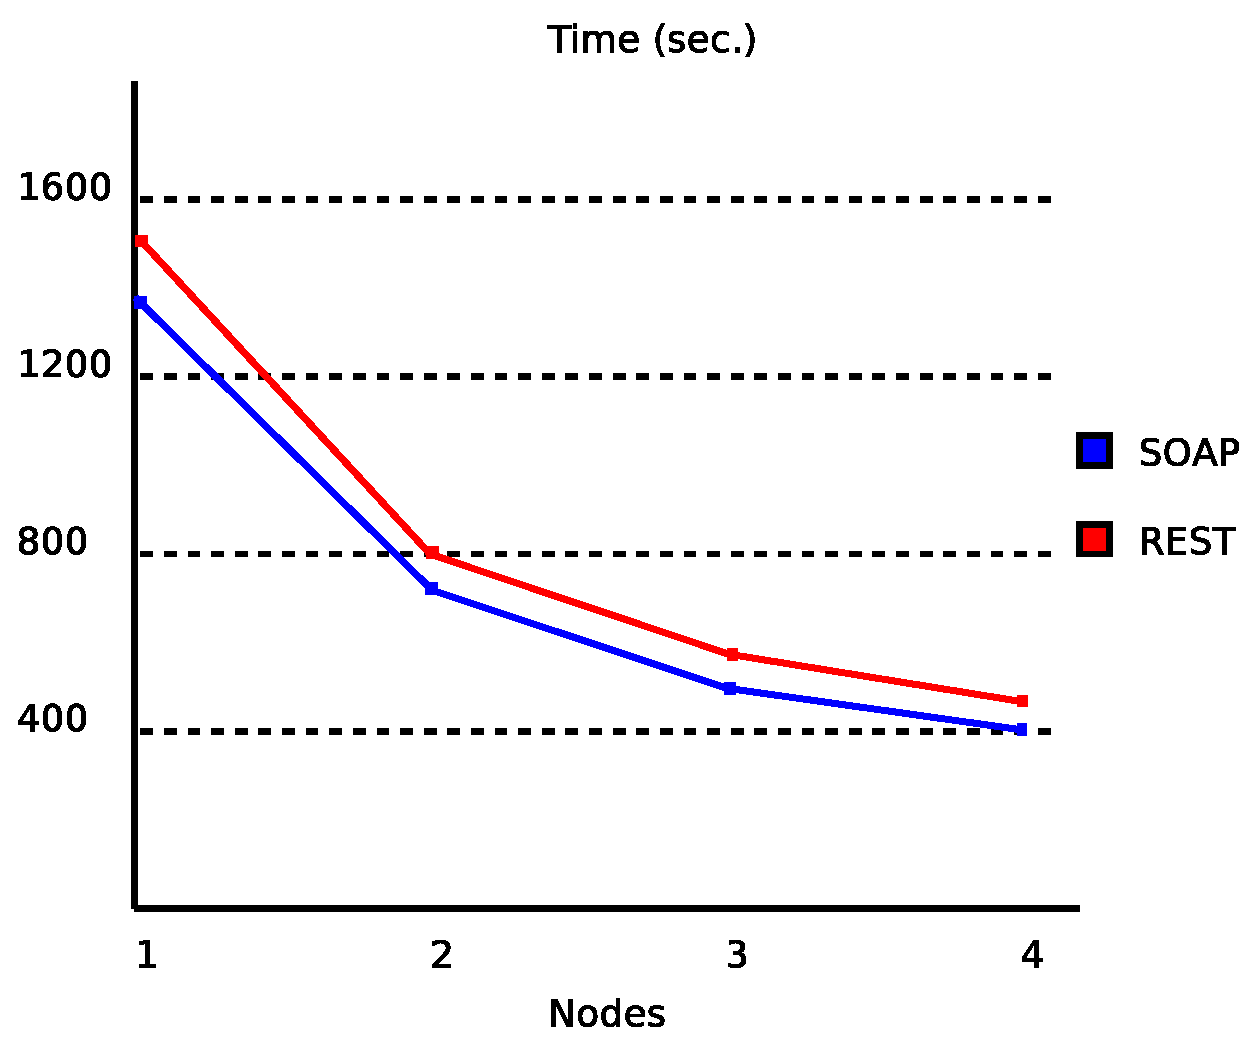
\epsfig{file=exp3_time.eps,width=8cm}
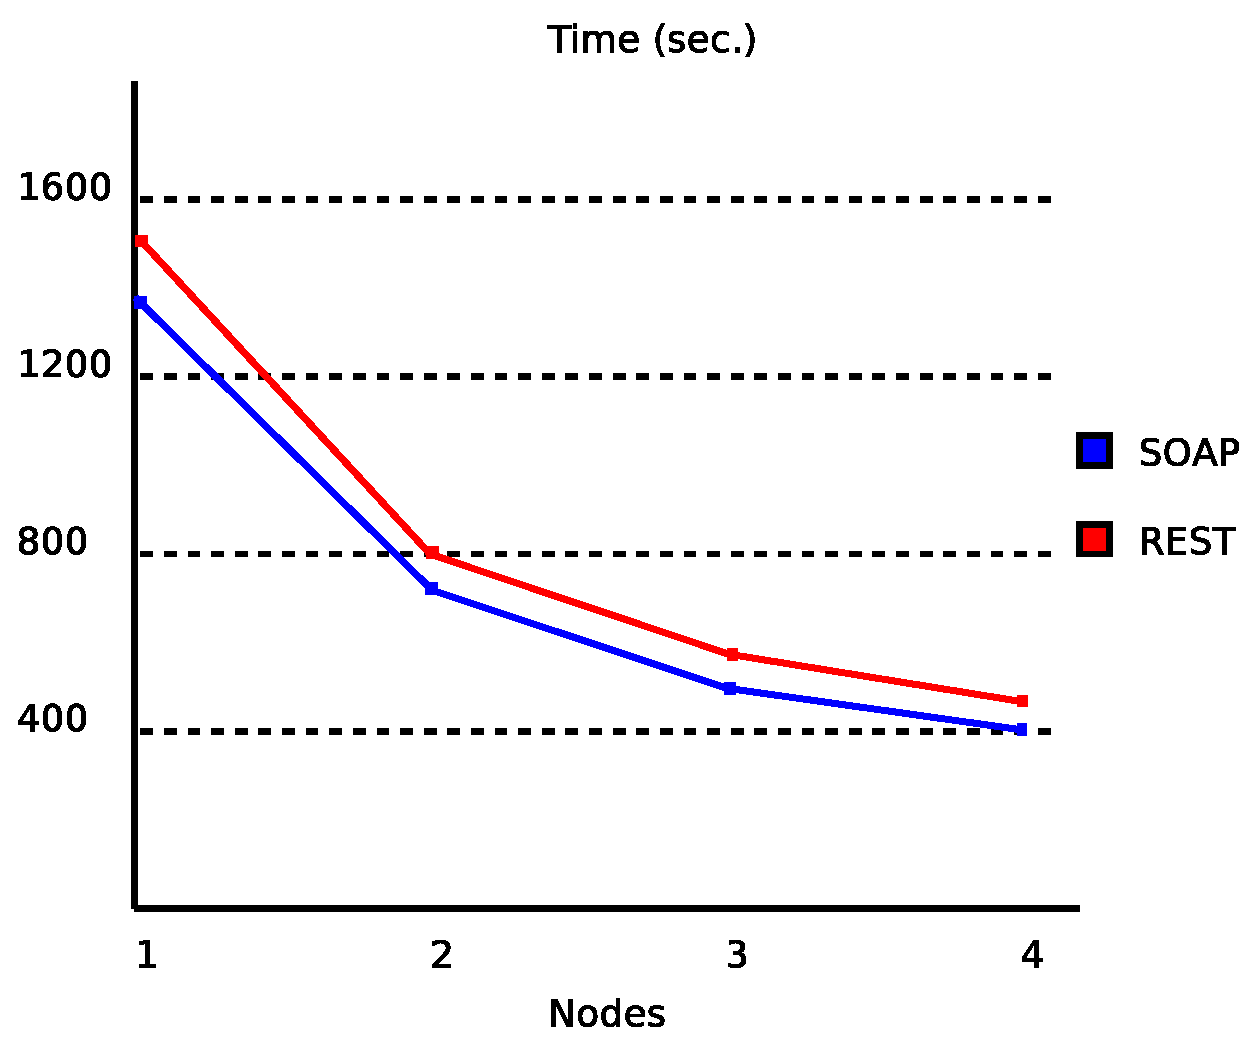
\includegraphics[width=8cm]{exp3_time.eps}
\caption{Plot of the running time (seconds) for both the SOAP and REST implementations. 
 % As can be seen, the REST version takes a slightly higher time as each communication takes longer than in the SOAP version (the message size is high in this experiment).
 }
\label{fig:resultados3time}
\end{center}
\end{figure}


Figure \ref{fig:ganancia} shows the speedup obtained in these runs. 
We can see that classification ability and running time can be improved dividing the problem between several processes that work in parallel.
Speedup does not equals the number of computers used; however, running time is improved using several computers. 
Thus, as adding new evaluators (heterogeneous computers running a Perl process) is an easy and costless task, we could take advantage of this system structure and flexibility to solve costly optimization problems.
In the case of SOAP implementation, speedup is slightly better than in the case of REST, due to the fact that SOAP communications are faster for big messages.


\begin{figure}[!ht]
\begin{center}
%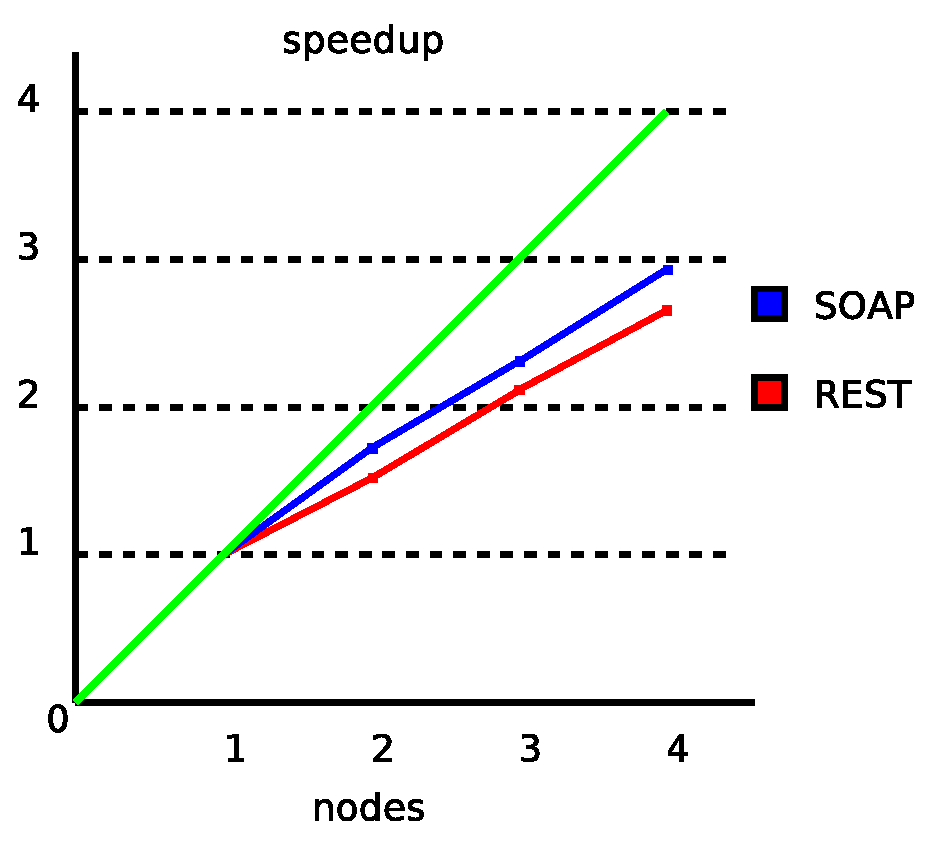
\epsfig{file=ganancia.eps,width=8cm}
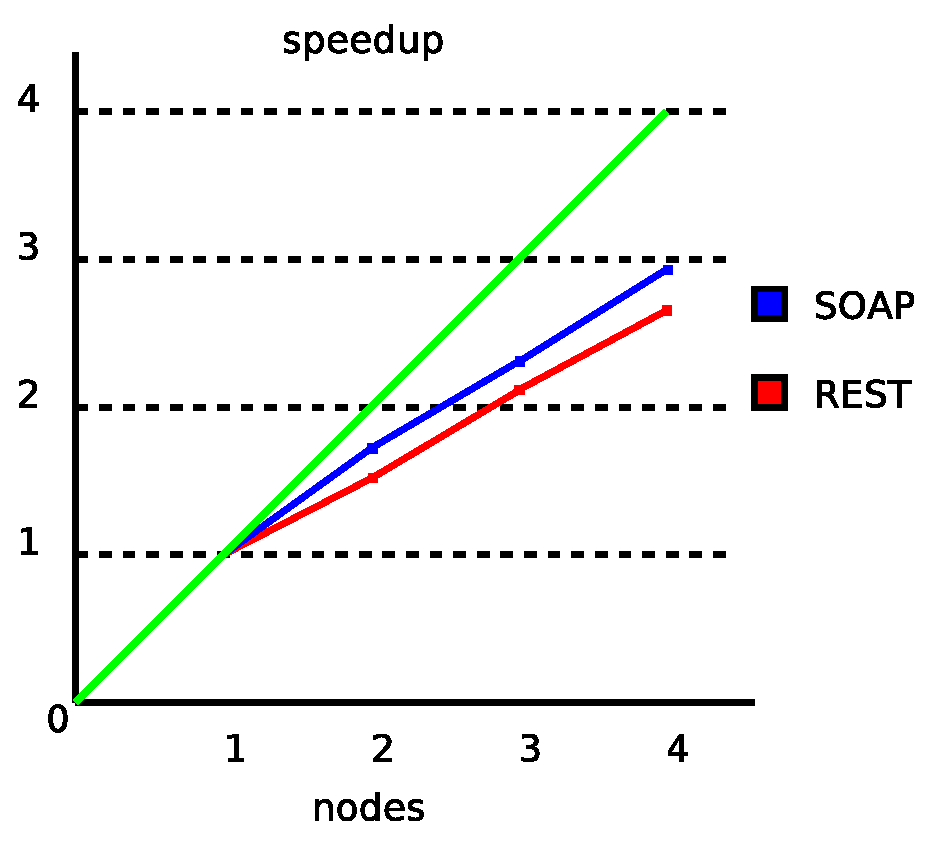
\includegraphics[width=8cm]{ganancia.eps}
\caption{Plot of the speedup obtained using SOAP and REST implementations, and $f(x) = x$ function (solid line). Although speedup is not lineal, it can be seen that running time is improved using several computers as clients dedicated to evaluate the individual fitness functions. 
 % REST-speedup is a bit lower compared to the SOAP one, due to the fact that REST version takes a slightly higher time.
}
\label{fig:ganancia}
\end{center}
\end{figure}


%As in this paper no improvement is made in terms of the algorithm, but in terms of the implementation and the technologies, we are not interested on comparing results against other authors. 
        % Esto pegaría en la respuesta, pero no aquí - JJ
%However, results obtained are comparable to those found in the bibliography \cite{Prechelt94c},\cite{MAG98},\cite{pedrajas2002_nn},\cite{catupaz2003},\cite{dzeroski2004},\cite{LeonBarranco2005},\cite{GarciaPedrajas2005},\cite{pedrajas2005_ieeetec} (see Table \ref{tabla:glass_resultados_OTROS}).
        % Y menos meter toda esa bibliografía. Yo me lo ventilaba  - JJ
%In some cases, authors report comparable errors on these problems \cite{domeniconi2000},\cite{pedrajas2002_nn},\cite{Wlodzislaw2004}, although no information on the experimental setup is given. Moreover, standard deviation is not reported, and therefore, no comparison can be made in order to apply statistical tests.   % to apply t-Student statistical tests.

%\begin{table}[!h] 
%\caption{Classification ability obtained using other methods for the Glass problem.}
%\label{tabla:glass_resultados_OTROS}
%\begin{tabular}{|c|c|c|c|c|c|}
%\hline %                domeniconi2000               Wlodzislaw2004           Wlodzislaw2004             pedrajas2005_ieeetec       pedrajas2002_nn
%\scriptsize{Scyth}   & \scriptsize{ADAMENN}      & \scriptsize{K-NN}      &  \scriptsize{C4.5}    &  \scriptsize{Coop.Ens.}     & \scriptsize{Dzeroski}  \\
%\scriptsize{\cite{domeniconi2000}}    & \scriptsize{\cite{domeniconi2000}}         & \scriptsize{\cite{Wlodzislaw2004}}      & \scriptsize{\cite{Wlodzislaw2004}}     &  \scriptsize{\cite{pedrajas2005_ieeetec}}          & \scriptsize{\cite{pedrajas2002_nn}}  \\
%\hline
%\scriptsize{27.1}    &    \scriptsize{24.8}      &   \scriptsize{28.0}    &  \scriptsize{31.8}    &   \scriptsize{22.9$\pm$4.8} & \scriptsize{25.2}  \\
%\hline
%\hline
%\hline% prechelt1994            MAG98                 LeonBarranco2005              GarciaPedrajas2005             pedrajas2002_nn             catupaz2003
%\scriptsize{Prechelt} & \scriptsize{Gr\"{o}nroos} & \scriptsize{ARGEN+}    & \scriptsize{Cascade}        &\scriptsize{MOBNET}      & \scriptsize{Cantú-Paz} \\
%\scriptsize{\cite{Prechelt94c}}     & \scriptsize{\cite{MAG98}}         & \scriptsize{AREPO\cite{LeonBarranco2005}} & \scriptsize{Ens.\cite{GarciaPedrajas2005}}       &\scriptsize{\cite{pedrajas2002_nn}}        & \scriptsize{\cite{catupaz2003}} \\
%\hline
%\scriptsize{32.08}    &  \scriptsize{32$\pm$0.5}  &  \scriptsize{32.33}    & \scriptsize{27$\pm$3}       &\scriptsize{29.6$\pm$3.1}& \scriptsize{32.9} \\
%\hline
%\end{tabular}
%\end{table}



%%%%%%%%%%%%%%%%%%%%%%%%%%%%%%%%%%%%%%%%%%%%%%%%%%%%%%%%%%%%%%%%%%%%%%%%%%%%%%%%
\section{Conclusions}
\label{sec:conclusionsAndFutureWork}

This paper presents a new parallel-distributed computation implementation using SOAP and REST web services that shows the useful these technologies can be in the field of evolutionary computation.

As reported in the experiments provided, both techniques are suitable for developing parallel systems.
However, depending on the amount of data sent, one might be heavier than the other.
On another hand, REST technology could not be used to implement a distributed GA following the island model as it does not support asynchronous processing and invocation, while SOAP does support it.

As seen, to implement and use communications using SOAP and REST it is not necessary running virtual machines (as in Java programming), nor daemons, just only to install several libraries available for almost any programming language.
Moreover, an arbitrary number of computers (clients-evaluators) can be added to the system, making it faster.

In these experiments, we have demonstrated that both can be used as communication protocol for distributed evolutionary computation, obtaining a good speedup.
Results obtained are comparable, and only for big messages, REST communications take longer than SOAP communications.
Differences in time between the proposed approaches are significant after the application of t-Student statistical tests.
They provide a common interface that can be called from almost any programming language and under any platform, taking advantage of their flexibility, fault tolerance and resilience to infrastructure breakdowns.
Thus, programs can be written in any language and can share data without the need of worrying about the message formats or communication protocols. 


Using REST and SOAP could increase the network overload, mainly because the headers size. 
For example, minimum header size in SOAP is 314 bytes (HTTP headers and SOAP envelope). 
However, this amount of data does not overload the network; moreover, in the case of sending a large number of data, this header size represents a small percentage of the total. 
On another hand, using either SOAP or REST provides several advantages: Protocols such as SOAP provide access to services. Besides, using the standard HTTP ports also skips network and firewall configuration (no new ports need to be open). Thus, SOAP and REST should be used in case the data to transmit is large enough (such as the experiments presented), where the header size is a small percentage of the data sent.
In any case, while running these experiments, no overload on the network was noticed (no delays in communications).
%At the same time, it does not overload too much the network.
Using other distributed systems, such as Jini \cite{jiniFAQ},\cite{Jini:FEA2000}, the network traffic is so high that when a high number of computers are used, communication becomes difficult.



\medskip

From these implementations, several paths for improvement are devised: 
changing the models so that more computation is moved to the clients, leaving the server as just a hub for information interchange among clients; that information interchange will have to be reduced to the minimum. That will make this model closer to the island model, with just the migration policies regulated by the server. That way, the server bottleneck is almost eliminated. 


Finally, it is necessary to use flexible tools that allow EA researchers to take advantage of all  available computation nodes, and make possible the self-adaptation of EAs in every execution environment and for each problem type. 
In this sense, the EA researchers should start to consider a migration from their actual software to be accessed as services.
Thus, as future research, it could be of interest adding support for SOAP and REST to existing distributed evolutionary algorithm libraries, such as JEO \cite{maribel:jp2001}, EO \cite{EOEA01}, and libraries in other languages, in order to allow the implementation of multi-language evolutionary algorithms.
%In these experiments, Perl language has been used. It could be interesting to test these technologies using other programming languages and libraries (i.e. Java).
Another possibility is to test P2P architectures, where each computer communicates only with one or two computers in the network. 
It would be very interesting to parallelize the proposed method using random topologies, in such a way that a ''servent'' (server/client) can enter or leave the network at any moment.



%%%%%%%%%%%%%%%%%%%%%%%%%%%%%%   AGRADECIMIENTOS  %%%%%%%%%%%%%%%%%%%%%%%%%%%%%%
\section*{Acknowledgements}

This work has been supported in part by 
%the Junta de Andaluc\'{\i}a {SIPEsCa} (G-GI3000/IDIF) project,
the P08-TIC-03903 project awarded by the Andalusian Regional Government
and 
the TIN2011-28627-C04-02 project.
%The authors are grateful to anonymous referees for their constructive comments and advice about the first version of our paper.
%The authors are very grateful to the anonymous referees whose comments and suggestions have contributed to improve this paper.


%%%%%%%%%%%%%%%%%%%%%%%%%%%%%%%%%%%%%%%%%%%%%%%%%%%%%%%%%%%%%%%%%%%%%%%%%%%%%%%%%%%%%%%%%
%%%%%%%%%%%%%%%%%%%%%%%%%%%%%%%%%%%%%%%%%%%%%%%%%%%%%%%%%%%%%%%%%%%%%%%%%%%%%%%%%%%%%%%%%
%%%%%%%%%%%%%%%%%%%%%%%%%%%%%%%%%%%%%%%%%%%%%%%%%%%%%%%%%%%%%%%%%%%%%%%%%%%%%%%%%%%%%%%%%

\bibliographystyle{plain} % elsarticle-num   spmpsci   spphys   spbasic
\bibliography{rest,geneura,gprop,javi,otras}

\end{document}

